\documentclass[11pt]{article}

% -----------------------------------------------------------------------------
% Paper: PX4Lockstep.jl simulator description (code-faithful)
% -----------------------------------------------------------------------------

\usepackage[margin=1in]{geometry}
\usepackage{amsmath,amssymb,mathtools}
\usepackage{booktabs}
\usepackage{microtype}
\usepackage{graphicx}
\usepackage{xcolor}
\usepackage{hyperref}
\usepackage[nameinlink,noabbrev]{cleveref}
\usepackage{siunitx}
\usepackage{enumitem}
\usepackage{tabularx}
\usepackage{listings}
\usepackage[section]{placeins}
\lstdefinelanguage{toml}{
  morecomment=[l]{\#},
  morestring=[b]",
  sensitive=true,
}
\lstset{
  basicstyle=\ttfamily\footnotesize,
  columns=fullflexible,
  breaklines=true,
  breakatwhitespace=true,
  showstringspaces=false,
  frame=single,
  framerule=0.2pt,
  rulecolor=\color{black!20},
  backgroundcolor=\color{black!6},
  aboveskip=0.8\baselineskip,
  belowskip=0.6\baselineskip,
}

\usepackage{tikz}
\usetikzlibrary{arrows.meta,positioning,shapes.geometric}

\hypersetup{colorlinks=true, linkcolor=blue!50!black, citecolor=blue!50!black, urlcolor=blue!50!black}
\setlength{\emergencystretch}{2em}

% -----------------
% Notation helpers
% -----------------
% Render code-ish identifiers without manual escaping and with decent line breaks.
\newcommand{\code}[1]{\nolinkurl{#1}}
\newcommand{\vect}[1]{\mathbf{#1}}
\newcommand{\mat}[1]{\mathbf{#1}}
\newcommand{\qbn}{\mat{q}_{bn}} % Body->NED quaternion
\newcommand{\Rbn}{\mat{R}_{bn}} % Body->NED DCM
\newcommand{\cross}{\times}

\title{PX4Lockstep.jl: Deterministic PX4 Lockstep SITL with a Julia-Owned Hybrid Simulation Engine}
\author{Bharat Tak\\Wingtra AG\\\texttt{bharat.tak@wingtra.com}}
\date{\today}

\begin{document}
\maketitle

\begin{abstract}
\noindent
\code{PX4Lockstep.jl} is a PX4 lockstep SITL driver and integration harness that connects independently developed component models (plant, power, environment, scenarios, estimator models, and uORB interfaces) into a single, executable closed-loop system. PX4 is advanced through a minimal C ABI on an injected integer-microsecond clock, while Julia owns the hybrid simulation timeline, continuous plant integration, environment forcing, scenario orchestration, and structured logging.

A key goal is system-level evaluation across operating conditions. The environment is modeled explicitly (atmosphere with altitude-dependent pressure, density, and temperature; gravity; and wind/turbulence), and scenarios provide repeatable command and fault sequences. This enables assessing vehicle and controller performance under a range of conditions, and it supports rapid ``what changed?'' experiments by swapping individual components (or their parameters) and observing the impact on other subsystems and on end-to-end outcomes.

Deterministic scheduling and record $\to$ replay are treated as enabling tools for debugging and regression: when executed in a controlled environment (single-threaded execution, pinned dependency versions, and seeded RNGs for stochastic sources), experiments can be reproduced and plant-side changes can be compared against recorded traces.

This paper is \emph{code-faithful}: it documents the implementation directly from the source (equations, defaults, and corner cases) and summarizes current verification coverage and the evaluation plan.
\end{abstract}

\clearpage
\renewcommand{\contentsname}{Table of Contents}
\tableofcontents
\clearpage

\section{Scope, terminology, and design goals}
\label{sec:intro}

This paper documents \code{PX4Lockstep.jl}, a PX4 lockstep SITL driver and hybrid drone simulator written in Julia. The implementation has two coupled layers:
\begin{enumerate}[leftmargin=*]
  \item a thin Julia wrapper around \code{libpx4\_lockstep} that steps PX4 on an injected integer-microsecond clock and publishes/subscribes uORB messages, and
  \item a deterministic Julia simulation stack that owns the hybrid timeline, plant dynamics, environment, scenarios, and logging.
\end{enumerate}

\subsection{Conceptual model}
\label{sec:intro-conceptual}

\Cref{fig:conceptual} shows the conceptual organization. The runtime engine advances an integer-microsecond event axis. At each event boundary it executes discrete-time \emph{sources} (scenario, wind, estimator, PX4 lockstep) to update a held \code{SimBus}. The continuous plant integrates between boundaries under sample-and-hold inputs constructed from the bus. Algebraic \emph{derived outputs} (e.g., battery telemetry) are evaluated at boundaries and published into the bus for PX4 and for logging.

\begin{figure}[t]
  \centering
  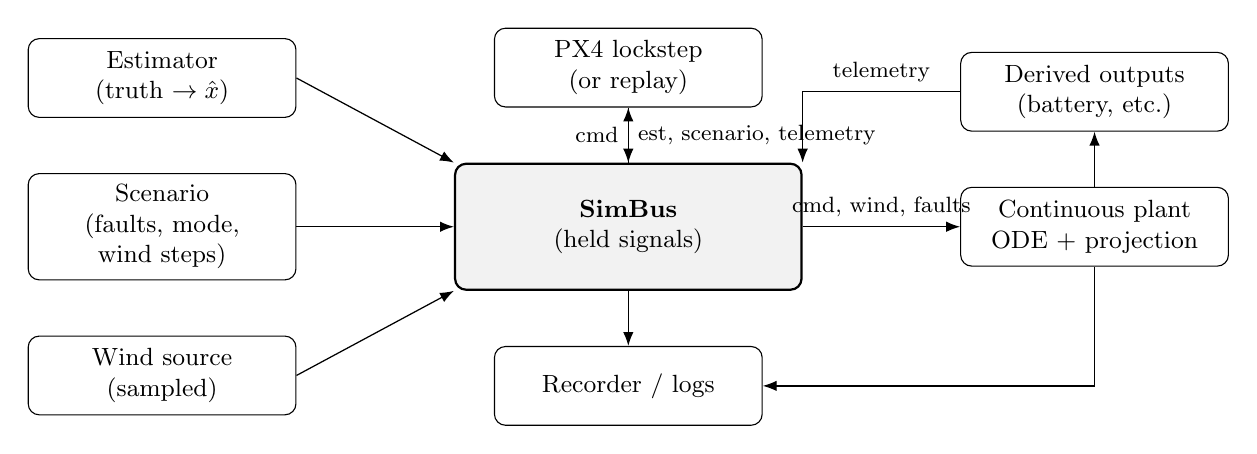
\begin{tikzpicture}[
      font=\small,
      >=Latex,
      node distance=7mm and 20mm,
      box/.style={draw, rounded corners, align=center, minimum width=34mm, minimum height=10mm, inner sep=4pt},
      bus/.style={draw, thick, rounded corners, fill=gray!10, align=center, minimum width=44mm, minimum height=16mm, inner sep=4pt},
      arr/.style={-Latex, line width=0.45pt}
    ]
    \node[bus] (bus) {\textbf{SimBus}\\(held signals)};

    % Left column: discrete sources (stacked to avoid overlap)
    \node[box, left=of bus] (scenario) {Scenario\\(faults, mode,\\wind steps)};
    \node[box, above=of scenario] (est) {Estimator\\(truth $\to \hat{x}$)};
    \node[box, below=of scenario] (wind) {Wind source\\(sampled)};

    % Top: PX4
    \node[box, above=of bus] (px4) {PX4 lockstep\\(or replay)};

    % Right column: plant + derived outputs
    \node[box, right=of bus] (plant) {Continuous plant\\ODE + projection};
    \node[box, above=of plant] (outputs) {Derived outputs\\(battery, etc.)};

    % Bottom: logging
    \node[box, below=of bus] (log) {Recorder / logs};

    % Discrete sources into the bus (use distinct anchors so arrows don't merge).
    \draw[arr] (est.east) -- (bus.north west);
    \draw[arr] (scenario.east) -- (bus.west);
    \draw[arr] (wind.east) -- (bus.south west);

    % PX4 reads from the bus and writes commands back.
    \draw[arr] (bus.north) -- node[midway, right]{\footnotesize est, scenario, telemetry} (px4.south);
    \draw[arr] (px4.south) -- node[midway, left]{\footnotesize cmd} (bus.north);

    % Plant reads held inputs.
    \draw[arr] (bus.east) -- node[midway, above]{\footnotesize cmd, wind, faults} (plant.west);

    % Derived outputs published back to the bus (route via the top to avoid overlaps).
    \draw[arr] (plant.north) -- (outputs.south);
    \draw[arr] (outputs.west) -| node[pos=0.25, above]{\footnotesize telemetry} (bus.north east);

    % Logging reads both.
    \draw[arr] (bus.south) -- (log.north);
    \draw[arr] (plant.south) |- (log.east);
  \end{tikzpicture}
  \caption{Conceptual structure. The engine schedules discrete sources on an integer-microsecond event axis and integrates the continuous plant between boundaries under sample-and-hold inputs.}
  \label{fig:conceptual}
\end{figure}

\subsection{Terminology and conceptual layering}
\label{sec:intro-terms}

The codebase is modular, but the paper uses a small number of terms consistently. \Cref{tab:terminology} defines the ones needed to reason about determinism.

\begin{table}[t]
  \centering
  \small
  \begin{tabularx}{\linewidth}{@{}lX@{}}
    \toprule
    Term & Meaning in this paper (as implemented) \\
    \midrule
    time axis & A sorted vector of integer microseconds owned by one subsystem (e.g., PX4 tick times, wind tick times). Built by \code{Runtime.Timeline} (\code{src/sim/Runtime/Timeline.jl}). \\
    event axis & The sorted unique union of all time axes. The engine integrates only on this axis. \\
    boundary & A specific event time $t_k$ where discrete sources may update the bus and where logging may occur. \\
    source & A discrete-time component with \code{Runtime.update!(src, bus, plant, t\_us)} (scenario, wind source, estimator, PX4 wrapper, replay samplers). \\
    bus & A mutable packet \code{Runtime.SimBus} holding piecewise-constant signals (cmd, wind, faults, estimates, telemetry) between boundaries. \\
    plant & The continuous-time state integrated by the engine: rigid body plus (optionally) actuator, rotor, and power states (\cref{sec:plant-state}). \\
    derived outputs & Algebraic outputs computed from the current plant state and held inputs at boundaries via \code{plant\_outputs(...)} (e.g. battery telemetry). \\
    \bottomrule
  \end{tabularx}
  \caption{Terminology and conceptual layering used throughout the paper.}
  \label{tab:terminology}
\end{table}

\subsection{Design goals and reader takeaways}
\label{sec:intro-goals}

The primary goal is not maximum physics fidelity; it is \emph{reviewable determinism} for controller-in-the-loop experiments:
\begin{itemize}[leftmargin=*]
  \item \textbf{Deterministic scheduling:} all boundary times are integer microseconds and the engine advances on an explicit union event axis.
  \item \textbf{Hybrid semantics:} discrete sources update only at event boundaries; the plant integrates with sample-and-hold inputs between boundaries.
  \item \textbf{Minimal trust boundary:} PX4 runs as a black box behind the lockstep ABI; all ``truth'' models live in Julia.
  \item \textbf{Reproducible analysis:} closed-loop runs can be recorded and replayed deterministically to compare plant-side changes.
\end{itemize}

Even if a reader never opens the repository, the intended takeaways are the four invariants below, which jointly define the execution model:
\begin{enumerate}[leftmargin=*]
  \item \textbf{Integer time contract:} all subsystem cadences and delays are exact multiples of \SI{1}{\micro\second} (otherwise the code errors).
  \item \textbf{Fixed boundary protocol:} all discrete updates at $t_k$ occur in a single canonical order (\cref{sec:runtime-boundary}), producing one well-defined bus value \code{bus(t\_k)}.
  \item \textbf{Sample-and-hold integration:} the plant integrates over $[t_k,t_{k+1}]$ using a single held input packet derived from \code{bus(t\_k)}.
  \item \textbf{Record/replay falsifiability:} boundary-aligned traces are recorded and replayed with exact axis alignment, enabling deterministic open-loop plant comparisons (\cref{sec:record-replay}).
\end{enumerate}

Whenever a statement below depends on a specific implementation choice, we point to the corresponding Julia entrypoint (module/function) rather than relying on prose in repository documentation. All file paths are written relative to the \code{px4\_lockstep\_julia} repository root.

\section{Deterministic runtime engine}
\label{sec:runtime}

The canonical run loop is \code{Sim.Runtime.Engine} (\code{src/sim/Runtime/Engine.jl}). It advances an integer-microsecond timeline, calls discrete-time \emph{sources} at event boundaries, and integrates the continuous-time plant between boundaries.

\subsection{Timebase and hybrid event timeline}
\label{sec:runtime-timebase}

All scheduling uses integer microseconds (\code{UInt64}). The helper \code{dt\_to\_us(dt\_s)} (\code{src/sim/Runtime/Timeline.jl}) converts a \code{Float64} interval in seconds to microseconds with an exactness requirement:
\begin{equation}
  \left|dt\_s - 10^{-6}\,\mathrm{round}(10^{6} dt\_s)\right| \le 10^{-15}.
\end{equation}
If the conversion is not exact (i.e. the requested interval is not an integer multiple of \SI{1}{\micro\second}), the code throws.

\paragraph{Timeline axes.}
The runtime constructs several named time axes, each a sorted vector of microseconds (\code{src/sim/Runtime/Timeline.jl}): autopilot ticks, wind ticks, logging ticks, scenario \emph{AtTime} boundaries, and an optional ``physics'' axis. The global event axis is the sorted unique union of all axis times, including both endpoints. The engine always integrates on this union axis: any subsystem boundary becomes an integration boundary.

\begin{figure}[!htbp]
  \centering
  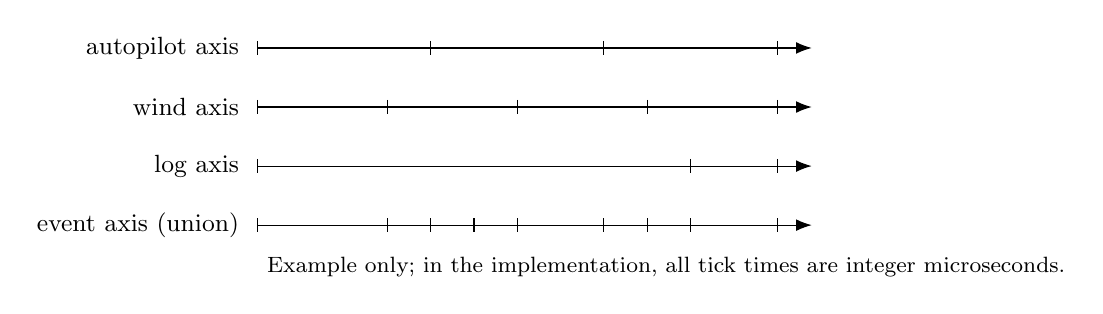
\begin{tikzpicture}[x=0.55cm,y=0.75cm, font=\small]
    \def\xmax{12}

    % Axis baselines
    \foreach \y/\name in {3/{autopilot axis},2/{wind axis},1/{log axis},0/{event axis (union)}} {
      \draw[-{Latex[length=2mm]}] (0,\y) -- (\xmax+0.8,\y);
      \node[anchor=east] at (-0.2,\y) {\name};
    }

    % Example tick sets (arbitrary units; the real code uses UInt64 microseconds).
    \foreach \t in {0,4,8,12} {\draw (\t,3+0.12) -- (\t,3-0.12);}
    \foreach \t in {0,3,6,9,12} {\draw (\t,2+0.12) -- (\t,2-0.12);}
    \foreach \t in {0,10,12} {\draw (\t,1+0.12) -- (\t,1-0.12);}
    \foreach \t in {0,3,4,5,6,8,9,10,12} {\draw (\t,0+0.12) -- (\t,0-0.12);}

    \node[anchor=west] at (0,-0.7) {\footnotesize Example only; in the implementation, all tick times are integer microseconds.};
  \end{tikzpicture}
  \caption{Multi-rate scheduling: each subsystem owns a time axis, and the engine integrates on their union (the event axis).}
  \label{fig:timeline-union}
\end{figure}

\subsection{TOML configuration: timeline axes}
\label{sec:runtime-toml}

The timeline parameters described above are configured in the \code{[timeline]} block of the aircraft spec (\code{TimelineSpec} in \code{src/sim/Aircraft/Spec.jl}, parsed by \code{src/sim/Aircraft/TOMLIO.jl}):

\begin{lstlisting}[language=toml]
[timeline]
t_end_s = 20.0
dt_autopilot_s = 0.004
dt_wind_s      = 0.001
dt_log_s       = 0.01
dt_phys_s      = 0.001  # optional; omit (or set to null) to disable extra physics boundaries
\end{lstlisting}

\paragraph{Parameter semantics (what the code does).}
\begin{itemize}[leftmargin=*,itemsep=2pt]
  \item \code{t\_end\_s}: inclusive simulation horizon. The engine always starts at \(t_0=0\) and forces both \(t_0\) and \(t_{end}\) into the union event axis.
  \item \code{dt\_autopilot\_s}: cadence of the autopilot axis (PX4 stepping, estimator publication, plant discontinuities).
  \item \code{dt\_wind\_s}: cadence of the wind axis. Wind is updated only on these ticks and held between them.
  \item \code{dt\_log\_s}: cadence of logging ticks. The implementation additionally appends a final log sample at \(t_{end}\) even when \(dt_{log}\) does not evenly divide the horizon (\code{build\_timeline}).
  \item \code{dt\_phys\_s}: optional additional periodic boundaries. When omitted, the ``physics'' axis degenerates to \(\{t_0,t_{end}\}\) and does not add boundaries beyond the other axes.
\end{itemize}

\paragraph{Mapping to the engine axes.}
Each interval is converted to integer microseconds by \code{dt\_to\_us} (\cref{sec:runtime-timebase}), giving
\begin{equation}
  \Delta t_{ap} \leftrightarrow \texttt{dt\_autopilot\_s},\quad
  \Delta t_{wind} \leftrightarrow \texttt{dt\_wind\_s},\quad
  \Delta t_{log} \leftrightarrow \texttt{dt\_log\_s},\quad
  \Delta t_{phys} \leftrightarrow \texttt{dt\_phys\_s}.
\end{equation}
Scenario \emph{AtTime} boundaries are \emph{not} configured in \code{[timeline]}; they are discovered from the scenario source via the \code{event\_times\_us} protocol hook and injected into the union axis by \code{build\_timeline\_for\_run}.

\subsection{Boundary protocol and sample-and-hold semantics}
\label{sec:runtime-boundary}

At each event time $t_k$ the engine executes boundary stages in a fixed canonical order (\code{src/sim/Runtime/BoundaryProtocol.jl}, applied by \code{process\_events\_at!} in \code{src/sim/Runtime/Engine.jl}):
\begin{enumerate}[leftmargin=*,itemsep=2pt]
  \item \textbf{Scenario}: update high-level commands (arm/mission/RTL), landed flag, faults, and optional wind disturbances.
  \item \textbf{Wind}: if the wind axis is due, step the wind source and publish the held \code{bus.wind\_ned} sample.
  \item \textbf{Derived outputs}: if the plant implements \code{plant\_outputs}, evaluate algebraic outputs (notably battery telemetry) and publish them into the bus.
  \item \textbf{Estimator}: if the autopilot axis is due, publish \code{bus.est} (truth injection + noise/bias/delay).
  \item \textbf{Telemetry}: optional deterministic inspection hooks (autopilot-axis only).
  \item \textbf{Autopilot}: if the autopilot axis is due, step PX4 (or replay) and publish \code{bus.cmd}.
  \item \textbf{Plant discontinuities}: if the autopilot axis is due, apply boundary-time plant updates (notably snapping \emph{direct} actuators via \code{plant\_on\_autopilot\_tick}).
  \item \textbf{Logging}: if the log axis is due, record a pre-step snapshot and emit structured logs.
\end{enumerate}

\paragraph{Why this order?}
The boundary protocol is part of the simulator semantics, not an implementation detail. At each boundary \(t_k\) the engine applies a discrete transition
\[
  (\mathrm{bus}_{k^-}, x_k) \;\xrightarrow{\;\text{boundary stages}\;}\; (\mathrm{bus}_{k^+}, x_k^+),
\]
where \(x_k\) is the continuous plant state at the boundary and \(x_k^+\) includes any boundary-time discontinuities (e.g.\ actuator snaps). The held plant input over the next interval is then defined by
\[
  u_k \coloneqq \mathrm{PlantInput}(\mathrm{bus}_{k^+}),\qquad
  u(t)=u_k\ \text{for}\ t\in[t_k,t_{k+1}).
\]
Reordering stages changes which signals are held over which intervals and therefore changes the meaning of the simulation.

The chosen ordering enforces the following invariants at PX4 ticks:
\begin{itemize}[leftmargin=*,itemsep=2pt]
  \item \textbf{No stale estimator inputs:} when the autopilot axis is due, PX4 consumes an estimator packet constructed from truth at the same boundary time \(t_k\).
  \item \textbf{No stale telemetry:} algebraic telemetry (e.g.\ battery status) is computed from \((t_k,x_k,u_k)\) and published before stepping PX4, so uORB injection reflects the current plant state.
  \item \textbf{Command-to-physics causality:} PX4 is stepped exactly once at \(t_k\), producing the unique command \(u_k\) that is held over \([t_k,t_{k+1})\).
  \item \textbf{Snap-after-command:} boundary-time discontinuities are applied after \code{bus.cmd} is published, so snapped actuator state is a deterministic function of the newly produced command.
  \item \textbf{Logs correspond to integration inputs:} logging occurs last so a snapshot at \(t_k\) corresponds to the same bus packet that seeds integration over \([t_k,t_{k+1})\).
\end{itemize}

Changing this ordering is therefore a semantic change (not ``just refactoring''): for example, stepping PX4 before the estimator would make PX4 consume a stale estimate; logging before PX4 would decouple recorded commands from the plant inputs that followed.

\paragraph{Scenario cadence.}
The scenario stage is currently executed at \emph{every} boundary on the union event axis, not only on the scenario axis. This makes hybrid \code{When(...)}-style logic responsive at the earliest possible boundary while preserving deterministic ordering (see the note in \code{src/sim/Runtime/BoundaryProtocol.jl} and the implementation in \code{process\_events\_at!}).

\paragraph{Wind disturbance consistency.}
If the scenario updates an additive wind disturbance at a boundary where the wind axis is \emph{not} due, the engine applies the disturbance delta immediately to the held wind sample so the piecewise-constant wind input remains consistent across axes.

\paragraph{Sample-and-hold.}\label{sec:runtime-sample-hold}
Between event times, all bus values are treated as sample-and-hold. The plant is integrated over $[t_k, t_{k+1})$ with a single input packet
\begin{equation}
  u_k \coloneqq \{\text{actuator command},\; \text{wind},\; \text{fault state}\},
\end{equation}
constructed from the bus at $t_k$ (\code{PlantInput} in \code{src/sim/Plant.jl}).


\subsection{Integration stepping and post-step projection}

Let $x(t)$ be the continuous plant state and $f(t, x, u)$ the plant RHS functor. At each interval the engine calls
\begin{equation}
  x_{k+1} \gets \mathrm{Integrate}(f,\, t_k,\, x_k,\, u_k,\, \Delta t_k)
\end{equation}
where $\Delta t_k = (t_{k+1}-t_k)\,10^{-6}$ seconds, and the integrator is selected by the aircraft spec (\code{src/sim/Integrators.jl}, \code{src/sim/Aircraft/Build.jl}).

\paragraph{Hybrid interval integration (contact-aware plants).}
\label{sec:runtime-hybrid-integrators}
Most plants can be advanced by calling \code{Integrators.step\_integrator} once per union-axis interval. Ground contact, however, is inherently hybrid: touchdown and liftoff introduce discontinuities that are not representable as a smooth ODE without either (i) stiff penalty forces or (ii) explicit event handling. The runtime therefore supports an optional protocol hook
\begin{quote}\small
\code{plant\_integrate\_interval(model, integrator, t0\_us, x0, u, dt\_us)}
\end{quote}
(\code{src/sim/PlantInterface.jl}). When implemented, the engine delegates the \emph{entire} interval advance to this method.

\paragraph{Free flight vs.\ contact-constrained stepping (current ground-contact implementation).}
For the coupled multirotor plant, \code{plant\_integrate\_interval} is implemented when \code{PlantSpec.contact} is \code{FlatGroundConstraintContact}. The interval integrator acts as a deterministic regime switcher:
\begin{itemize}[leftmargin=*,itemsep=2pt]
  \item \textbf{Airborne segments (smooth dynamics):} the plant is advanced under the \emph{free} dynamics \(f_{\mathrm{free}}\) (the same model but with \code{NoContact()}) using the configured integrator (RK4/RK23/RK45, etc.). Near the ground, the next airborne chunk can be capped to \(O(\text{time-to-impact})\) so that a descending crossing of the guard is bracketed reliably.
  \item \textbf{Impact events (discontinuous map):} if a lookahead airborne chunk brackets a descending crossing of \(z=0\), the TOI is localized to integer microseconds by deterministic bisection and an impact map is applied at that internal time (position projection + velocity reset with restitution and optional tangential friction). Multiple impacts can be handled inside one outer interval, but the code caps the count to a fixed maximum to avoid pathological bounce storms.
  \item \textbf{Grounded segments (constraint/impulse stepping):} while the state is a ground candidate, the plant advances in fixed substeps of \code{h\_contact\_us}. Each substep uses a single evaluation of \(f_{\mathrm{free}}\) (explicit Euler) followed by a closed-form, 1-contact impulse solve (normal + Coulomb friction) and a position-only stabilization on \(z\). In this grounded regime the configured integrator is \emph{not} used; the time-stepping loop is deliberately fixed-step and deterministic.
\end{itemize}
The full contact math and the exact update equations are documented in \cref{sec:contacts-hybrid}.

\paragraph{Interval metadata and logging.}
Because impacts can occur at internal TOI times \(\tau\in(t_k,t_{k+1})\), the interval integrator may optionally return per-interval metadata (impact count, maximum \(\Delta v\), and its timestamp). The engine accumulates this metadata into latched bus signals for logging (\code{bus.impact\_dv\_ned}, \code{bus.impact\_time\_us}, \code{bus.impact\_count}) and also computes a simple ``equivalent acceleration'' estimate at the autopilot tick rate (\code{bus.impact\_accel\_est\_ned}); see \code{Runtime.Engine.\_accumulate\_interval\_impacts!}.

Some state variables have hard physical bounds (e.g. rotor speed $\omega \ge 0$, battery SOC in $[0,1]$). The engine therefore supports an optional post-step projection hook \code{plant\_project(model, x)} that clamps or projects state deterministically after each accepted interval. The coupled multirotor plant implements this projection (\code{src/sim/PlantModels/CoupledMultirotor.jl}).

\paragraph{Record $\to$ replay (high level).}
The same engine can run in a mode that records boundary-aligned bus/plant streams, and a replay mode that replaces ``live'' sources with trace samplers. This converts a closed-loop PX4 run into a deterministic open-loop plant replay for integrator/model comparisons.

\begin{figure}[t]
  \centering
  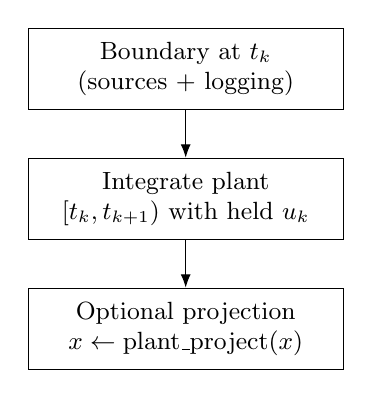
\begin{tikzpicture}[
      node distance=6mm and 10mm,
      font=\small,
      box/.style={draw, align=center, minimum width=40mm, inner ysep=5pt, inner xsep=6pt},
      arr/.style={-Latex, line width=0.4pt}
    ]
    \node[box] (b) {Boundary at $t_k$\\(sources + logging)};
    \node[box, below=of b] (i) {Integrate plant\\$[t_k, t_{k+1})$ with held $u_k$};
    \node[box, below=of i] (p) {Optional projection\\$x \leftarrow \mathrm{plant\_project}(x)$};
    \draw[arr] (b) -- (i);
    \draw[arr] (i) -- (p);
  \end{tikzpicture}
  \caption{Engine rhythm: boundary processing on the union event axis, then continuous plant integration over the next interval under sample-and-hold inputs.}
  \label{fig:engine-rhythm}
\end{figure}

\section{Determinism contract, threat model, and evaluation plan}
\label{sec:determinism}

The runtime in \cref{sec:runtime} makes the execution model explicit. This section (i) defines what ``determinism'' means for this project, (ii) states a threat model for when the claim is defensible, and (iii) summarizes what is already verified in the repository and what remains to be evaluated.

\subsection{What ``determinism'' means here}
\label{sec:determinism-definition}

We use ``determinism'' in a concrete, falsifiable sense: for a fixed initial plant state, a fixed simulation specification, a fixed integer-microsecond timeline, and fixed seeds for any stochastic sources, the simulator should produce boundary-aligned traces that are \emph{numerically identical within tight tolerances} across repeated runs in a controlled software/hardware environment. Bitwise identity is a stronger property that is only expected under strict runtime controls (single-threaded execution, pinned dependencies, and stable CPU/libm); we therefore treat bitwise identity as a best-case outcome rather than the baseline contract.

More specifically, the codebase targets three nested determinism properties:
\begin{enumerate}[leftmargin=*]
  \item \textbf{Scheduling determinism:} the same set of event times \(\{t_k\}\) is generated from the same configuration, and the engine visits them in a deterministic order (\cref{sec:runtime-timebase}).
  \item \textbf{Discrete-source determinism:} for each boundary time \(t_k\), each source publishes an unambiguous bus update in a fixed stage ordering (\cref{sec:runtime-boundary}).
  \item \textbf{Numerical determinism:} given the same held inputs and floating-point execution environment, the plant integration produces the same state at each boundary time (up to tight tolerances).
\end{enumerate}

The first two properties are architectural and are largely ``by construction'' once time is represented as integer microseconds. The third property depends on floating-point behavior and library/environment controls.

\subsection{Mechanisms used in the implementation}
\label{sec:determinism-mechanisms}

The implementation contains several explicit mechanisms intended to make determinism reviewable:
\begin{itemize}[leftmargin=*]
  \item \textbf{Integer-microsecond timebase:} all axes are stored as \code{UInt64} microseconds and the timeline builder rejects non-exact cadences (\code{dt\_to\_us}; \cref{sec:runtime-timebase}).
  \item \textbf{Union event axis:} the engine integrates only on the sorted unique union of subsystem axes, so a discrete update can never occur ``inside'' an integration step (\cref{fig:timeline-union}).
  \item \textbf{Fixed boundary protocol:} a single canonical stage ordering defines what the autopilot consumes and what input is held over the next interval (\cref{sec:runtime-boundary}).
  \item \textbf{Sample-and-hold bus:} all plant inputs are derived from a held \code{SimBus} packet at boundaries (\cref{sec:runtime-sample-hold}).
  \item \textbf{Dedicated RNG ownership for stochastic sources:} live wind and live estimator sources carry their own RNG instances and document the rule ``no RNG usage outside of \code{update!}'' (\code{src/sim/Sources/Wind.jl}, \code{src/sim/Sources/Estimator.jl}).
  \item \textbf{Deterministic iteration counts in key algebraic solvers:} the coupled plant bus-voltage solve uses staged deterministic strategies with fixed iteration counts (\cref{sec:bus-solve}).
  \item \textbf{Axis-aligned record/replay:} recorded streams are validated to match their intended axes exactly (\code{_require\_axis\_match!}), and replay sources sample by deterministic binary search over the recorded axis vectors (\cref{sec:record-replay}).
  \item \textbf{Microsecond-quantized adaptive substeps:} adaptive Runge--Kutta integrators optionally quantize accepted substeps to integer microseconds (\code{quantize\_us=true} by default in \code{src/sim/Integrators.jl}) to reduce drift from floating time accumulation.
\end{itemize}

\subsection{TOML configuration: deterministic seeding}
\label{sec:determinism-toml-seed}

All stochastic sources are expected to be seeded explicitly through the aircraft spec. The seed is configured under \code{[aircraft]}:

\begin{lstlisting}[language=toml]
[aircraft]
name = "iris"   # optional human-readable identifier
seed = 1        # integer seed for deterministic RNG ownership
\end{lstlisting}

\paragraph{Parameter semantics (what the code does).}
\begin{itemize}[leftmargin=*,itemsep=2pt]
  \item \code{name}: used only for identification/logging; it does not affect dynamics.
  \item \code{seed}: used to seed deterministic RNGs during build. In the default builder (\code{src/sim/Aircraft/Build.jl}), the wind source uses \code{seed} and the noisy estimator uses \code{seed+1}. If \code{seed} is not specified, \code{AircraftSpec()} defaults to \code{1}.
\end{itemize}

This is a narrow but explicit contract: deterministic randomness requires the simulator to own the RNG state and to treat seeds as part of the experiment configuration.


\subsection{Threat model for determinism}
\label{sec:determinism-threat-model}

Even with a deterministic execution model, determinism can be undermined by factors outside the scheduling layer. The paper therefore makes an explicit threat model:

\paragraph{In-scope (what the design intends to control).}
\begin{itemize}[leftmargin=*]
  \item Discrete-event ordering and held-input semantics (fully controlled by the engine).
  \item RNG-based sources, provided they use dedicated RNG state and fixed seeds (controlled by the source constructors and aircraft spec).
  \item Data-dependent loop termination, where the code uses fixed-iteration schemes for critical algebraic steps (e.g. bus solve) or where floating-point decisions are deterministic given a fixed environment.
\end{itemize}

\paragraph{Out-of-scope / risks (must be controlled by the run harness or explicitly disclaimed).}
\begin{itemize}[leftmargin=*]
  \item \textbf{Threading and nondeterministic reductions.} The simulator is intended to run single-threaded, but the code does not enforce this globally. Any multi-threaded dependency (e.g. BLAS, linear algebra kernels, reductions) can introduce nondeterministic floating-point association.
  \item \textbf{Cross-platform floating-point differences.} Bitwise identity across CPU architectures, OS/libm versions, or compiler flags is not guaranteed in IEEE 754 arithmetic. The project currently targets repeatability within a controlled environment; cross-platform repeatability should be treated as an empirical question.
  \item \textbf{Dependency drift.} If package versions change (Julia version, \code{Manifest.toml} content), numerical behavior can change even if the code is unchanged.
  \item \textbf{Iteration order and hash stability.} Determinism can be broken by unordered iteration (e.g.\ \code{Dict} traversal) or randomized hashing across Julia versions. The implementation avoids unordered iteration in core loops; any new code must be careful about iteration order.
  \item \textbf{Math flags and fused operations.} Compiler flags or macros such as \code{@fastmath} can enable reassociation or fused-multiply-add, which may change results across platforms or builds. These are avoided in the core simulation path.
  \item \textbf{Sorting stability assumptions.} Any use of sorting as a deterministic tie-breaker must guarantee a stable order and explicit keying; otherwise equal keys can lead to nondeterministic outcomes across versions.
  \item \textbf{PX4 black-box behavior.} PX4 is treated as an external component. While lockstep stepping removes wall-clock timing drift, internal PX4 behavior can still depend on floating-point implementation details and configuration.
\end{itemize}

\paragraph{Required controls for determinism claims.}
To make determinism claims academically defensible, runs intended for determinism evaluation \emph{must} satisfy the following:
\begin{itemize}[leftmargin=*]
  \item set \code{JULIA\_NUM\_THREADS=1} and disable BLAS threading (e.g. \code{OPENBLAS\_NUM\_THREADS=1}, \code{MKL\_NUM\_THREADS=1}, \code{VECLIB\_MAXIMUM\_THREADS=1}),
  \item execute with the repository's \code{Project.toml} and \code{Manifest.toml} pinned (no dependency drift),
  \item use explicit seeds for any live stochastic sources (wind, noisy estimator), and
  \item report the Julia version, OS, CPU, and relevant environment variables alongside results.
\end{itemize}

\subsection{Evidence already present in the repository}
\label{sec:determinism-evidence}

Even without an ``evaluation'' section with plots, the repository already contains regression tests that operationalize determinism at the trace level:
\begin{itemize}[leftmargin=*]
  \item \code{test/record\_replay\_engine.jl} constructs minimal plants and asserts:
    (i) replay integration matches an analytic solution for a piecewise-constant input,
    (ii) record mode captures axis-aligned Tier-0 traces, and
    (iii) record \(\to\) reload \(\to\) replay reproduces the logged plant state at every log tick to tight tolerances (position/velocity/attitude/body-rate/rotor/battery terms on the order of \(10^{-12}\) or smaller). This is the operative determinism contract in the current test suite.
  \item \code{test/compare\_integrators.jl} runs deterministic integrator sweeps on a fixed recording, validating solver ordering and error metric wiring.
  \item Multiple unit tests validate model components that directly influence determinism (e.g. battery surface interpolation and scaling, motor mapping, and gyro/rotor sign conventions).
\end{itemize}

These tests are limited (short horizon, controlled scenarios), but they provide a concrete starting point: determinism is checked by comparing boundary-aligned traces, not by subjective visual similarity.

\begin{figure}[t]
  \centering
  \includegraphics[width=\linewidth]{figs/determinism_drift.png}
  \caption{Determinism check: two replay runs of the same recording using the same integrator (RK4) produce negligible drift over 700\,s.}
  \label{fig:determinism-drift}
\end{figure}

\begin{figure}[t]
  \centering
  \includegraphics[width=0.7\linewidth]{figs/replay_rtf_long.png}
  \caption{Replay-only realtime factor for a 700\,s Iris mission recording (no PX4 calls during the replay sweep). Run configuration is summarized in \cref{app:run-context}.}
  \label{fig:replay-rtf}
\end{figure}

\subsection{Evaluation plan (results to be added)}
\label{sec:determinism-eval-plan}

A ``proper'' paper version should extend the above test-style checks into a small evaluation section. The following experiments can be added without changing the architecture:
\begin{enumerate}[leftmargin=*]
  \item \textbf{Replay fidelity (closed-loop \(\to\) open-loop):} record a short closed-loop mission, then replay the plant using the recorded \code{:cmd}, \code{:wind\_base\_ned}, and scenario traces, and report that Tier-0 log streams match within tolerance.
  \item \textbf{Repeated-run determinism:} run the same recording replay multiple times and verify identical Tier-0 outputs within tolerance (optionally also report bytewise hashes when strict controls are used).
  \item \textbf{Cross-machine repeatability (if feasible):} replay the same Tier-0 file on a second machine/OS and report drift envelopes, explicitly noting whether results are bitwise-identical or only numerically close.
  \item \textbf{Cost trade-offs:} measure wall-clock overhead as a function of event-axis density (union-axis refinement), log cadence, and adaptive-integrator tolerance.
  \item \textbf{Sensitivity to numerical choices:} use the existing integrator sweep tooling (\cref{sec:record-replay}) to report how solver choice changes plant trajectories under identical recorded inputs, and quantify the effect of \code{quantize\_us} on adaptive error control.
\end{enumerate}

Where the current implementation makes arbitrary choices (e.g. fixed iteration counts, simple contact model, simplified aero), those choices should be stated as such and evaluated for their impact on determinism, stability, and fidelity rather than defended as universally correct.

\section{Evidence summary (current repository)}
\label{sec:evidence-summary}

The full validation results are presented later (\cref{sec:validation}), but a short summary here anchors the key claims early:
\begin{itemize}[leftmargin=*,itemsep=2pt]
  \item \textbf{Determinism replay drift:} two replay runs of the same recording produce negligible drift over 700\,s (\cref{fig:determinism-drift}).
  \item \textbf{Replay performance:} replay-only realtime factor for a 700\,s mission is summarized in \cref{fig:replay-rtf} (no PX4 calls during replay).
  \item \textbf{Integrator verification:} analytic/invariant checks for SHO, pendulum, Kepler, and torque-free rigid-body cases are tabulated in \cref{tab:verification-analytic-results}.
  \item \textbf{Record/replay sweep:} end-to-end Iris record/replay integrator sweep errors are reported in \cref{tab:verification-iris-sweep}.
\end{itemize}

These results are intentionally lightweight but they are executable and traceable to scripts in the repository, making them suitable as regression anchors.

\section{Frames and sign conventions}
\label{sec:frames}

The simulator follows PX4's conventional world frame:
\begin{itemize}[leftmargin=*,itemsep=2pt]
  \item \textbf{World/inertial frame}: NED (North--East--Down). Position and velocity are stored as $\vect{p}_{ned}$ and $\vect{v}_{ned}$ in meters and m/s.
  \item \textbf{Body frame}: FRD (Forward--Right--Down). Angular rate is stored as $\vect{\omega}_{body}=(p,q,r)$ in rad/s.
\end{itemize}

\subsection{Quaternion convention}

Attitude is stored as a unit quaternion \(\qbn\) representing the rotation \emph{Body $\to$ NED} in $(w,x,y,z)$ order (\code{src/sim/Types.jl}). The corresponding direction cosine matrix is denoted \(\Rbn\) (\code{quat\_to\_dcm}).

The rigid-body kinematic equation implemented in \code{src/sim/RigidBody.jl} is
\begin{equation}
  \dot{\qbn} = \tfrac{1}{2}\,\qbn \otimes \begin{bmatrix}0 \\ \vect{\omega}_{body}\end{bmatrix},
\end{equation}
where $\otimes$ is the Hamilton product (\code{quat\_mul}). Quaternions are explicitly normalized during state updates to limit numerical drift.


\subsection{Home origin and NED-to-LLA injection}
\label{sec:home-origin}

Several parts of the simulator (atmosphere sampling and PX4 uORB state injection) require converting local NED coordinates into latitude/longitude/altitude (LLA). The implementation uses a \emph{spherical Earth} small-angle approximation with a fixed radius \(R_E=\) \code{EARTH\_RADIUS\_M} \(=6.378137\times 10^6\,\si{m}\) (\code{src/sim/Autopilots.jl}):
\begin{align}
  \Delta\varphi &= \frac{p_{ned,x}}{R_E}, &
  \Delta\lambda &= \frac{p_{ned,y}}{R_E\cos(\mathrm{deg2rad}(\varphi_0))},\\
  \varphi &= \varphi_0 + \mathrm{rad2deg}(\Delta\varphi), &
  \lambda &= \lambda_0 + \mathrm{rad2deg}(\Delta\lambda),\\
  h_{msl} &= h_0 - p_{ned,z},
\end{align}
where \((\varphi_0,\lambda_0,h_0)\) is the configured home origin and \(p_{ned,z}\) is positive down.

\paragraph{Validity range.}
This flat-Earth approximation is intended for local missions on the order of \(\sim\)\SI{10}{km} from the home origin. Longitude uses a fixed \(\cos(\varphi_0)\) scale factor and altitude is linear; large-area navigation requires a geodesic model. See \cref{sec:design-choices} for the rationale and extension plan.

\paragraph{Radius consistency note.}
For LLA injection we use the WGS84 equatorial radius (\(R_E=6.378137\times 10^6\,\si{m}\)). The default spherical-gravity model now uses the same value (via \code{Autopilots.EARTH\_RADIUS\_M}) for \code{gravity\_r0\_m} in the environment spec (\cref{sec:environment}). Both are configurable if a different convention is required.

\paragraph{Angle units.}
Throughout the codebase, fields named \code{*\_deg} are stored in degrees. When a trigonometric function is applied to a \code{*\_deg} value, the implementation uses degree-aware functions (e.g.\ \code{cosd}) or an explicit \code{deg2rad} conversion. This is done at the call site, not globally; readers should assume trig is in radians unless a \code{*d} helper or an explicit \code{deg2rad} appears.

\paragraph{TOML configuration.}
The home origin is configured via the \code{[home]} block (\code{Types.WorldOrigin}, aliased as \code{Autopilots.HomeLocation}):

\begin{lstlisting}[language=toml]
[home]
lat_deg    = 47.397742
lon_deg    = 8.545594
alt_msl_m  = 488.0
\end{lstlisting}

\paragraph{Parameter mapping.}
\begin{itemize}[leftmargin=*,itemsep=2pt]
  \item \code{lat\_deg} \(\rightarrow \varphi_0\) in degrees.
  \item \code{lon\_deg} \(\rightarrow \lambda_0\) in degrees.
  \item \code{alt\_msl\_m} \(\rightarrow h_0\) in meters above mean sea level.
\end{itemize}
These parameters affect only coordinate conversions and altitude-dependent environment queries; they do not change the local NED rigid-body dynamics directly.

\subsection{Propulsor axis convention}
\label{sec:axis-convention}

Each propulsor $i$ has a unit axis vector $\vect{a}_{b,i}$ expressed in body/FRD axes. See \code{Vehicles.PropulsorLayout} and \code{Vehicles.QuadrotorParams}. The thrust force applied to the rigid body is defined as
\begin{equation}
  \vect{F}_{b,i} = -T_i\,\vect{a}_{b,i},
\end{equation}
so the ``typical'' multirotor case (thrust along \(-\)body-$z$) uses \(\vect{a}_{b,i}=(0,0,1)\). Rotor axes from specs are normalized during aircraft build (\code{src/sim/Aircraft/Build.jl}).

The propulsion layer produces a signed reaction torque magnitude per rotor. The rigid-body model applies it as a moment about the propulsor axis:
\begin{equation}
  \vect{\tau}_{b,i}^{\text{reaction}} = Q_i\,\vect{a}_{b,i}.
\end{equation}

\paragraph{Rotor direction bookkeeping.}
The multirotor configuration distinguishes:
\begin{itemize}[leftmargin=*,itemsep=2pt]
  \item \code{rotor\_dir[i]}: the \emph{reaction torque sign on the body} used to sign $Q_i$.
  \item Rotor spin direction: opposite to the reaction torque sign (used for rotor gyroscopic coupling, \cref{sec:rigid-body}).
\end{itemize}

\section{Continuous-time plant state and integrators}
\label{sec:plant-state}

The engine integrates a \emph{full plant state} rather than only rigid-body states. This makes variable-step integration meaningful: actuator dynamics, rotor-speed dynamics, and battery dynamics are integrated alongside the rigid body.

\subsection{Plant state and held input packet}

The rigid-body state (\code{RigidBodyState} in \code{src/sim/RigidBody.jl}) is
\begin{equation}
  x_{rb} \coloneqq \{\vect{p}_{ned},\; \vect{v}_{ned},\; \qbn,\; \vect{\omega}_{body}\}.
\end{equation}

The full continuous plant state (\code{PlantState} in \code{src/sim/Plant.jl}) extends this with actuator and powertrain states:
\begin{align}
  x \coloneqq \{&x_{rb},\; \vect{y}_m,\; \dot{\vect{y}}_m,\; \vect{y}_s,\; \dot{\vect{y}}_s,\; \vect{\Omega},\; \text{power}\},\\
  &\vect{y}_m\in\mathbb{R}^{12},\; \vect{y}_s\in\mathbb{R}^{8},\; \vect{\Omega}\in\mathbb{R}^{N}.
\end{align}
Motor/servo outputs are stored in fixed-size arrays to match the PX4 lockstep ABI (12 motor channels, 8 servo channels), while $N$ is the number of \emph{physical} propulsors.

The plant consumes a piecewise-constant input packet (\code{PlantInput}) held over each engine interval:
\begin{equation}
  u \coloneqq \{\mathtt{cmd},\; \vect{w}_{ned},\; \mathtt{faults}\},
\end{equation}
where \texttt{cmd} is the latest actuator command, $\vect{w}_{ned}$ is the latest sampled wind velocity, and \texttt{faults} is a compact fault mask (e.g. motor disable bitmask, battery connected flag).

\subsection{Fixed-step and adaptive integrators}
\label{sec:integrators}

The integrators in \code{src/sim/Integrators.jl} are dependency-light and operate directly on \code{RigidBodyState} or \code{PlantState}:
\begin{itemize}[leftmargin=*,itemsep=2pt]
  \item \textbf{Euler}: forward Euler (debug).
  \item \textbf{RK4}: classic fixed-step 4th-order Runge--Kutta.
  \item \textbf{RK23}: Bogacki--Shampine 3(2) with adaptive step.
  \item \textbf{RK45}: Dormand--Prince 5(4) with adaptive step.
\end{itemize}

Adaptive methods compute an error estimate from the difference between the ``high'' and ``low'' order solutions. The default error norm is an $\ell_\infty$-style scaled maximum over rigid-body groups (position, velocity, body rates) plus a geodesic attitude error on $SO(3)$:
\begin{equation}
  e_q = \frac{2\arccos(|\langle q_{hi}, q_{lo}\rangle|)}{\max(\mathtt{atol\_att\_rad},\epsilon)}.
\end{equation}
By default, non-rigid-body plant states (actuator, rotor speed, battery) do \emph{not} influence adaptivity. Setting \code{plant\_error\_control=true} enables additional error terms provided the corresponding absolute tolerances are finite.

\paragraph{Microsecond quantization of adaptive substeps.}
Both adaptive integrators support \code{quantize\_us=true} (default), which quantizes internal substep sizes to integer microseconds to preserve the engine's integer-time contract. This is a determinism trade-off: quantization slightly perturbs the step-size controller and can degrade error-control optimality near stiff-ish dynamics (e.g.\ contact-adjacent transients). Its impact should be reported in evaluations.

\paragraph{Engine-level note.}
The engine resets integrator internal step-size history at the start of every event interval (\code{reset!(integrator)} inside \code{Engine.step\_to\_next\_event!}). This maximizes determinism isolation between intervals but may reduce adaptive efficiency compared to carrying history across intervals.


\subsection{TOML configuration: integrator selection and tolerances}
\label{sec:integrator-toml}

The integrator described in \cref{sec:integrators} is selected in the \code{[plant]} block (\code{PlantSpec.integrator}, parsed by \code{_parse\_integrator} in \code{src/sim/Aircraft/toml/Sections/Plant.jl}). The parser accepts either a string shorthand:
\begin{lstlisting}[language=toml]
[plant]
integrator = "RK4"   # "Euler" | "RK4" | "RK23" | "RK45"
\end{lstlisting}
or a table form for adaptive solvers with explicit tolerances:
\begin{lstlisting}[language=toml]
[plant]
integrator = { kind="RK45",
  rtol_pos=1e-7, atol_pos=1e-6,
  rtol_vel=1e-7, atol_vel=1e-6,
  rtol_omega=1e-7, atol_omega=1e-6,
  atol_att_rad=1e-6,
  plant_error_control=false,
  h_min=1e-6,
  max_substeps=50000,
  quantize_us=true
}
\end{lstlisting}

\paragraph{Parameter mapping to the adaptive error model.}
The tolerance keys map directly to the error computation used by RK23/RK45:
\begin{itemize}[leftmargin=*,itemsep=2pt]
  \item \code{rtol\_pos}, \code{atol\_pos}: relative/absolute tolerances for the position group \(\vect{p}_{ned}\).
  \item \code{rtol\_vel}, \code{atol\_vel}: relative/absolute tolerances for the velocity group \(\vect{v}_{ned}\).
  \item \code{rtol\_omega}, \code{atol\_omega}: tolerances for body rates \(\vect{\omega}_{body}\). (The TOML parser also accepts Unicode omega keys via TOML escapes, e.g.\ \verb|rtol_\u03C9| and \verb|atol_\u03C9|.)
  \item \code{atol\_att\_rad}: absolute tolerance for the attitude geodesic error \(e_q\) in \cref{sec:integrators}.
  \item \code{plant\_error\_control}: when \code{true}, include non-rigid-body plant states (actuators, rotor speed, SOC, \(v_1\), temperature) in the adaptive error norm if their absolute tolerances are finite.
\end{itemize}

\paragraph{Step-size controls.}
\begin{itemize}[leftmargin=*,itemsep=2pt]
  \item \code{h\_min}: lower bound on internal adaptive substeps (seconds).
  \item \code{max\_substeps}: hard cap on internal substeps per engine interval; exceeding it throws.
  \item \code{quantize\_us}: when \code{true}, accepted adaptive substeps are quantized to integer microseconds to reduce drift against the engine's integer-time axis (\cref{sec:runtime-timebase}).
\end{itemize}

Any omitted fields take constructor defaults from the selected integrator's constructor (\code{src/sim/Integrators.jl}).

\section{Rigid-body multirotor dynamics}
\label{sec:rigid-body}

The baseline vehicle model is \texttt{Sim.Vehicles.GenericMultirotor}, a rigid-body multirotor with configurable propulsor geometry. It is intentionally low-fidelity but allocation-free and stable for closed-loop testing.

\subsection{Translational dynamics}
The position derivative is simply
\begin{equation}
  \dot{\vect{p}}_n = \vect{v}_n.
\end{equation}

The total thrust force in body coordinates is formed by summing per-rotor thrust vectors. Each propulsor has a body-frame axis \(\vect{a}_{b,i}\) (\code{QuadrotorParams.rotor\_axis\_body}) with the convention
\begin{equation}
  \vect{F}_{b,i} = -T_i\,\vect{a}_{b,i},
\end{equation}
so for a classic multirotor with thrust along \(-z_b\), \(\vect{a}_{b,i}=(0,0,1)\). The total body force is
\begin{equation}
  \vect{F}_b = \sum_{i=1}^{N} \vect{F}_{b,i}, \qquad \vect{F}_n = \Rbn\,\vect{F}_b.
\end{equation}

A simple linear drag term is applied in NED based on air-relative velocity
\begin{equation}
  \vect{v}_{rel} = \vect{v}_n - \vect{w}_n, \qquad \vect{F}_{drag} = -c_d\,\vect{v}_{rel},
\end{equation}
where \(c_d\) is \code{QuadrotorParams.linear\_drag} and \(\vect{w}_n\) is the held wind sample from the runtime bus.

Finally, gravity is supplied by the environment model as an acceleration vector \(\vect{g}_n\) (positive down in NED). The velocity derivative is
\begin{equation}
  \dot{\vect{v}}_n = \frac{1}{m}\left(\vect{F}_n + \vect{F}_{drag}\right) + \vect{g}_n.
\end{equation}

\subsection{Rotational dynamics with rotor gyroscopics}
Moments from propulsors have two contributions: (i) thrust at a lever arm, and (ii) reaction torque about the propulsor axis. With body-frame rotor position \(\vect{r}_{b,i}\) and thrust \(T_i\),
\begin{equation}
  \vect{\tau} = \sum_{i=1}^{N} \left( \vect{r}_{b,i} \cross \vect{F}_{b,i} + \vect{a}_{b,i}\,\tau_i \right),
\end{equation}
where \(\tau_i\) is the signed shaft torque reported by the propulsion layer. In the current implementation this is the \emph{aerodynamic load torque} \(Q_i\) from the prop model, signed by \texttt{rotor\_dir[i]} (reaction torque on the body). Transient motor spin-up/spin-down effects enter separately through the rotor angular momentum terms \(-\dot{\vect{H}}\) and \(-\vect{\omega}_b \cross \vect{H}\); they are not double-counted inside \(\tau_i\).

The rigid-body angular dynamics include angular damping and the additional angular momentum stored in spinning rotors. Let \(\mat{I}\) be the body inertia, \(\vect{\omega}_b\) the body rates, and define the rotor angular momentum and its derivative
\begin{equation}
  \vect{H} = \sum_{i=1}^{N} J_i\,s_i\,\Omega_i\,\vect{a}_{b,i}, \qquad
  \dot{\vect{H}} = \sum_{i=1}^{N} J_i\,s_i\,\dot{\Omega}_i\,\vect{a}_{b,i},
\end{equation}
where \(J_i\) is the axial inertia of rotor \(i\), \(\Omega_i\) its spin rate (rad/s), and \(s_i=-\texttt{rotor\_dir}[i]\) is the rotor spin sign (opposite the reaction-torque sign). The implemented equation of motion is
\begin{equation}
  \mat{I}\,\dot{\vect{\omega}}_b = \left(\vect{\tau} - \vect{d}\odot\vect{\omega}_b\right)
  - \vect{\omega}_b\cross(\mat{I}\vect{\omega}_b)
  - \vect{\omega}_b\cross\vect{H} - \dot{\vect{H}},
\end{equation}
with elementwise angular damping \(\vect{d}\) from \code{QuadrotorParams.angular\_damping}. Quaternion kinematics use \cref{sec:frames}.

\begin{figure}[ht]
  \centering
  \includegraphics[width=0.75\linewidth]{figs/gyro_coupling_plot.png}
  \caption{Gyro coupling regression for a tilted rotor axis: expected vs simulated \(\dot{\omega}\) components.}
  \label{fig:gyro-coupling}
\end{figure}

\subsection{Defaults and caveats}
\paragraph{Defaults.} \code{QuadrotorParams} provides constructor defaults (used if a spec omits values): mass \SI{1.5}{kg}, diagonal inertia \((0.029125,0.029125,0.055225)\,\si{kg.m^2}\), linear drag \SI{0.05}{N/(m/s)}, and angular damping $(0.02,0.02,0.01)$.

\paragraph{Contact forces.} The rigid-body model itself does not include ground contact. Contact is handled in the coupled plant layer: penalty contact adds an external COM force in the RHS, while constraint contact can use hybrid interval stepping (time-of-impact + impact map + grounded impulses). See \cref{sec:contacts}.

\paragraph{Aerodynamics.} The drag term is deliberately simplistic (linear, isotropic, no lift/induced effects). This is appropriate for controller-in-the-loop regression but not for aerodynamic performance prediction.

\subsection{TOML configuration: airframe geometry and initial state}
\label{sec:airframe-toml}

The rigid-body parameters in \cref{sec:rigid-body} are configured under \code{[airframe]} (\code{AirframeSpec} in \code{src/sim/Aircraft/Spec.jl}) and its nested \code{[airframe.x0]} initial-condition table. A typical multirotor configuration (matching the shipped Iris asset) is:

\begin{lstlisting}[language=toml]
[airframe]
kind = "multirotor"
mass_kg = 1.5
inertia_diag_kgm2 = [0.029125, 0.029125, 0.055225]
# Optional products of inertia Ixy, Ixz, Iyz (defaults to zeros)
inertia_products_kgm2 = [0.0, 0.0, 0.0]

rotor_pos_body_m = [
  [ 0.1515,  0.2450, 0.0],
  [-0.1515, -0.1875, 0.0],
  [ 0.1515, -0.2450, 0.0],
  [-0.1515,  0.1875, 0.0],
]
rotor_axis_body_m = [
  [0.0, 0.0, 1.0],
  [0.0, 0.0, 1.0],
  [0.0, 0.0, 1.0],
  [0.0, 0.0, 1.0],
]

linear_drag = 0.05
angular_damping = [0.02, 0.02, 0.01]

[airframe.x0]
pos_ned    = [0.0, 0.0, 0.0]
vel_ned    = [0.0, 0.0, 0.0]
q_bn       = [1.0, 0.0, 0.0, 0.0]   # or euler_deg / euler_rad
omega_body = [0.0, 0.0, 0.0]
\end{lstlisting}

\paragraph{Parameter mapping to the dynamics.}
The keys above map one-to-one into the symbols used in \cref{sec:rigid-body}:
\begin{itemize}[leftmargin=*,itemsep=2pt]
  \item \code{mass\_kg} \(\rightarrow m\).
  \item \code{inertia\_diag\_kgm2} and \code{inertia\_products\_kgm2} \(\rightarrow\) the symmetric inertia tensor \(\mat{I}\). (Alternatively, \code{inertia\_kgm2} may be supplied as a full symmetric \(3\times 3\) tensor.)
  \item \code{rotor\_pos\_body\_m} \(\rightarrow \vect{r}_{b,i}\) for each rotor.
  \item \code{rotor\_axis\_body\_m} \(\rightarrow \vect{a}_{b,i}\) for each rotor. Axes are normalized during build; if omitted entirely, all axes default to \((0,0,1)\) (thrust along \(-z_b\)).
  \item \code{linear\_drag} \(\rightarrow c_d\) in \(\vect{F}_{drag}=-c_d\,\vect{v}_{rel}\).
  \item \code{angular\_damping} \(\rightarrow \vect{d}\) in \(\vect{d}\odot\vect{\omega}_b\).
\end{itemize}

\paragraph{Initial condition semantics.}
The \code{[airframe.x0]} table sets the initial rigid-body state. Attitude may be specified either as \code{q\_bn} or as Euler angles; in strict mode, only one representation may be supplied.

\section{Actuation and propulsion}
\label{sec:actuation-propulsion}

The canonical multirotor plant integrates actuator dynamics and propulsion dynamics inside one RHS (\code{Sim.PlantModels.CoupledMultirotorModel}) so that both fixed-step and adaptive integrators see a single continuous system.

\subsection{Actuator channel mapping and dynamics}

PX4 produces actuator commands as fixed-size ABI arrays: 12 motor channels in $[0,1]$ and 8 servo channels in $[-1,1]$ (\code{Vehicles.ActuatorCommand}). These are \emph{normalized lockstep ABI units} (not PWM) taken from the uORB outputs subscribed by the bridge (\code{actuator\_motors} and \code{actuator\_servos}); they are interpreted as normalized ESC duty and control-surface deflection. The plant stores actuator outputs in the same fixed-size arrays ($\vect{y}_m\in\mathbb{R}^{12}$, $\vect{y}_s\in\mathbb{R}^{8}$), but the physical vehicle may have $N\le 12$ propulsors.

\paragraph{Mapping from PX4 channels to physical motors.}
A typed mapping (\code{Vehicles.MotorMap\{N\}}) selects which PX4 motor channel drives each physical motor:
\begin{equation}
  d_i \coloneqq (\vect{y}_m)[\texttt{motor\_channel}[i]],\qquad i\in\{1,\dots,N\}.
\end{equation}
Faults are defined over \emph{physical} motors (indices $1..N$), not PX4 channels. The plant applies the motor-disable mask by forcing the affected physical duties to zero before evaluating propulsion.

\paragraph{Actuator dynamics.}
Actuator channel dynamics are integrated as part of the plant state. Motor and servo channels can each use one of the following models (\code{src/sim/Vehicles.jl}, \code{src/sim/PlantModels/CoupledMultirotor.jl}):
\begin{itemize}[leftmargin=*,itemsep=2pt]
  \item \textbf{Direct}: algebraic output, snapped to the new command at each autopilot boundary via \code{plant\_on\_autopilot\_tick}, then held.
  \item \textbf{First-order}: \(\dot{\vect{y}} = (\vect{u}_{cmd} - \vect{y})/\tau\).
  \item \textbf{Second-order}: \(\dot{\vect{y}}=\dot{\vect{y}}_{\mathrm{eff}}\), \(\ddot{\vect{y}}=\omega_n^2(\vect{u}_{cmd}-\vect{y})-2\zeta\omega_n\dot{\vect{y}}_{\mathrm{eff}}\), with an optional rate limit implemented by clamping \(\dot{\vect{y}}_{\mathrm{eff}}\) in the RHS and projecting stored rate states post-step.
\end{itemize}

After each engine interval the coupled plant implements \code{plant\_project} to clamp actuator outputs into ABI ranges and to project second-order rate states back into the configured rate limit, ensuring hard bounds are enforced deterministically.

\begin{figure}[t]
  \centering
  \includegraphics[width=\linewidth]{figs/actuator_step_response.png}
  \caption{Actuator step response example: direct vs second‑order dynamics with a rate limit.}
  \label{fig:actuator-step-response}
\end{figure}

\begin{figure}[t]
  \centering
  \includegraphics[width=\linewidth]{figs/motor_spinup.png}
  \caption{Motor/prop spin‑up example for a step duty command at constant bus voltage.}
  \label{fig:motor-spinup}
\end{figure}

\subsection{Motor/ESC/prop model}
\label{sec:propulsion-model}

Each physical motor uses a parameter-only container \code{Propulsion.MotorPropUnit} consisting of:
(i) an ESC stage with efficiency $\eta$ and deadzone, (ii) a quasi-static BLDC electrical model, and (iii) a quadratic propeller model with an inflow correction. The plant integrates rotor speed $\Omega_i$ (rad/s) for each physical motor.

\paragraph{ESC stage.}
The commanded duty is clamped to $[0,1]$ and zeroed if it is below the ESC deadzone. The motor terminal voltage is
\begin{equation}
  V_m = d\,V_{bus}.
\end{equation}

\paragraph{BLDC electrical model (quasi-static current).}
Let $K_v$ be specified in RPM/V. The back-EMF constant is
\begin{equation}
  K_e = \frac{60}{2\pi K_v} \quad \left[\mathrm{V}\,\mathrm{s}/\mathrm{rad}\right],
\end{equation}
and the torque constant is set equal to $K_t\equiv K_e$ (SI). Motor current is computed from applied voltage and back-EMF and then clamped:
\begin{equation}
  I_m = \mathrm{clamp}\!\left(\frac{V_m - K_e\,\Omega}{R},\; 0,\; I_{\max}\right).
\end{equation}
The electrical torque subtracts an approximate no-load current $I_0$:
\begin{equation}
  \tau_e = K_t\,\max(0, I_m - I_0).
\end{equation}

\paragraph{Loss modeling note.}
In this model, $I_0$ represents \emph{electrical} no-load current (iron/core loss) that does not produce torque, while $b\,\Omega$ is a \emph{mechanical} drag torque. The defaults are a pragmatic generic fit rather than a motor identification; if you want a single loss channel, set either $I_0=0$ (pure mechanical drag) or $b=0$ (pure electrical loss) to avoid double-counting.

\paragraph{Quadratic propeller aerodynamics.}
At air density $\rho$ the thrust and load torque are
\begin{equation}
  T = k_T\,\rho\,\Omega^2\,f_T(\mu),\qquad
  Q = k_Q\,\rho\,\Omega^2\,f_Q(\mu),
\end{equation}
with a simple inflow sensitivity factor
\begin{equation}
  f(\mu) = \frac{1}{1 + k\,\mu^2},\qquad \mu = \frac{V_{ax}}{\max(10^{-3}, |\Omega|R_{prop})}.
\end{equation}
The prop radius $R_{prop}$ is stored in the prop parameters. The coupled plant computes the axial component $V_{ax}$ by projecting the \emph{air velocity relative to the vehicle} onto each propulsor axis (\cref{sec:axis-convention}):
\begin{equation}
  \vect{v}_{air,n} = \vect{w}_{ned} - \vect{v}_{ned},\qquad
  \vect{v}_{air,b} = \Rbn^{\mathsf{T}}\,\vect{v}_{air,n},\qquad
  V_{ax,i} = -\vect{v}_{air,b}\cdot \vect{a}_{b,i}.
\end{equation}
The inflow correction uses $\mu^2$, so the sign of $V_{ax}$ affects neither $f_T$ nor $f_Q$. This $1/(1+k\mu^2)$ attenuation is an ad-hoc shaping term (not a blade-element or momentum-theory model) chosen for stability and simplicity; it cannot represent windmilling, vortex-ring, or braking regimes. See \cref{sec:design-choices}.

\paragraph{Rotor-speed dynamics.}
In the coupled plant, rotor speed is a continuous state integrated by the same ODE integrator as the rest of the plant. The RHS evaluates
\begin{equation}
  \dot{\Omega} = \frac{\tau_e - Q - b\,\Omega}{J},
\end{equation}
where $J$ is the axial inertia and $b$ is a viscous friction coefficient, and where $Q$ is the aerodynamic load torque evaluated at the \emph{current} $\Omega$ (no internal Euler step inside the RHS). A guard prevents unphysical negative spin: if $\Omega\le 0$ and $\dot{\Omega}<0$, the derivative is set to zero.

\paragraph{Bus current and signed reaction torque.}
The current drawn from the bus is
\begin{equation}
  I_{bus} = \frac{d\,I_m}{\max(10^{-6},\eta)}.
\end{equation}
The quadratic prop model returns a positive load torque magnitude $Q\ge 0$. The coupled plant applies a per-rotor sign \code{rotor\_dir[i]} to generate the signed reaction torque on the body,
\begin{equation}
  Q_{body,i} = \texttt{rotor\_dir}[i]\,Q_i,
\end{equation}
and passes this signed value into the rigid-body dynamics.

\subsection{Default propulsion parameterization and calibration}
\label{sec:propulsion-defaults}

The helper \code{Propulsion.default\_multirotor\_set} provides a generic baseline motor+prop set. It calibrates the thrust coefficient $k_T$ by solving for the steady-state speed at duty $d=1$ under a quadratic load and then bisection-searching $k_T$ so that the resulting thrust matches a target.

In the aircraft builder (\code{src/sim/Aircraft/Build.jl}), this target is derived from the airframe mass and gravity:
\begin{equation}
  T_{hover,rotor} = \frac{m\,g}{N},\qquad T_{target} = \texttt{thrust\_calibration\_mult}\cdot T_{hover,rotor},
\end{equation}
with \texttt{thrust\_calibration\_mult}=2.0 by default. The drag torque coefficient is tied to $k_T$ through \texttt{km\_m} via $k_Q = \texttt{km\_m}\,k_T$.

\paragraph{Caveat.}
This calibration is a pragmatic way to get reasonable thrust scaling for a ``generic'' vehicle. It is not an identification procedure for a specific airframe; if you care about realism beyond closed-loop controllability, replace the parameters with airframe-specific values.


\subsection{TOML configuration: actuation mapping and propulsion parameters}
\label{sec:actuation-toml}

Actuation and propulsion are configured in two places in the aircraft spec:
\begin{itemize}[leftmargin=*,itemsep=2pt]
  \item \code{[actuation]} defines how PX4 ABI channels map to physical motors/servos and which actuator dynamics model is used.
  \item \code{[airframe.propulsion]} defines the motor/ESC/prop parameters used by the coupled plant (\cref{sec:propulsion-model}).
\end{itemize}

A minimal Iris-like configuration is:

\begin{lstlisting}[language=toml]
[actuation]

[[actuation.motors]]
id = "motor1"
channel = 1

[[actuation.motors]]
id = "motor2"
channel = 2

[[actuation.motors]]
id = "motor3"
channel = 3

[[actuation.motors]]
id = "motor4"
channel = 4

[actuation.motor_actuators]
kind = "direct"   # direct | first_order | second_order

[actuation.servo_actuators]
kind = "direct"

[airframe.propulsion]
kind = "multirotor_default"
km_m = 0.05
V_nom = 12.0
rho_nom = 1.225
rotor_radius_m = 0.127
inflow_kT = 8.0
inflow_kQ = 8.0
thrust_calibration_mult = 2.0
rotor_dir = [1, 1, -1, -1]

[airframe.propulsion.esc]
eta = 0.98
deadzone = 0.02

[airframe.propulsion.motor]
kv_rpm_per_volt = 920.0
r_ohm = 0.25
j_kgm2 = 1.2e-5
i0_a = 0.6
viscous_friction_nm_per_rad_s = 2.0e-6
max_current_a = 60.0
\end{lstlisting}

\paragraph{Actuation mapping semantics.}
Each entry in \code{[[actuation.motors]]} creates a named physical motor ID and assigns it a PX4 channel index. During build, IDs are resolved into a \code{MotorMap\{N\}} so that \(\texttt{channel}\) implements the lookup in \cref{sec:actuation-propulsion}:
\[
  d_i \leftarrow (\vect{y}_m)[\texttt{channel}_i].
\]
Unknown IDs referenced elsewhere (e.g. by buses) are rejected at build time.

\paragraph{Actuator model parameters.}
The actuator model may be given as a string shorthand (\code{kind="direct"} etc) or as a table with parameters. For example, a second-order motor actuator with a finite rate limit uses:
\begin{lstlisting}[language=toml]
[actuation.motor_actuators]
kind = "second_order"
"\u03C9n" = 20.0   # omega_n
"\u03B6"  = 0.7    # zeta
rate_limit = 100.0   # units: (duty)/s
\end{lstlisting}
These keys map directly to \(\omega_n\), \(\zeta\), and the optional \(\dot{\vect{y}}\) clamp described in \cref{sec:actuation-propulsion}.

\paragraph{Propulsion parameter mapping.}
The propulsion keys match the symbols used in \cref{sec:propulsion-model}:
\begin{itemize}[leftmargin=*,itemsep=2pt]
  \item \code{kv\_rpm\_per\_volt} \(\rightarrow K_v\) (and thus \(K_e=60/(2\pi K_v)\) and \(K_t=K_e\)).
  \item \code{r\_ohm} \(\rightarrow R\) in \(I_m=(V_m-K_e\Omega)/R\).
  \item \code{i0\_a} \(\rightarrow I_0\) in \(\tau_e=K_t\max(0,I_m-I_0)\).
  \item \code{max\_current\_a} \(\rightarrow I_{\max}\) current clamp.
  \item \code{j\_kgm2} and \code{viscous\_friction\_nm\_per\_rad\_s} \(\rightarrow J\) and \(b\) in \(\dot{\Omega}=(\tau_e-Q-b\Omega)/J\).
  \item \code{eta} and \code{deadzone} configure the ESC stage (\cref{sec:propulsion-model}).
  \item \code{rotor\_radius\_m} \(\rightarrow R_{prop}\) in the inflow ratio \(\mu\).
  \item \code{inflow\_kT}, \code{inflow\_kQ} \(\rightarrow k\) in \(f(\mu)=1/(1+k\mu^2)\) for thrust and torque respectively.
  \item \code{km\_m} ties \(k_Q\) to \(k_T\) through \(k_Q=\texttt{km\_m}\,k_T\) in the default prop model.
  \item \code{thrust\_calibration\_mult} sets the target thrust multiplier used during build-time calibration (\cref{sec:propulsion-defaults}).
  \item \code{rotor\_dir[i]} signs the reaction torque applied to the body, \(Q_{body,i}=\texttt{rotor\_dir}[i]\,Q_i\). Rotor spin sign is the opposite (\(s_i=-\texttt{rotor\_dir}[i]\)) for gyroscopic coupling in \cref{sec:rigid-body}.
\end{itemize}

\section{Power network and battery models}
\label{sec:power}

The coupled multirotor plant solves battery-to-bus-to-motor coupling algebraically at each RHS evaluation and integrates battery internal states (SOC, polarization voltage, and optional temperature).

\subsection{Battery state and model families}
\label{sec:battery-model}

Battery state is part of \code{PlantState} as a \code{PowerState} with per-battery vectors:
\begin{equation}
  \text{power} = \{\vect{s}, \vect{v}_1, \vect{T}\},
\end{equation}
where $\vect{s}\in[0,1]^B$ is state-of-charge (fraction remaining), $\vect{v}_1\in\mathbb{R}^B$ is the Thevenin polarization voltage state, and $\vect{T}\in\mathbb{R}^B$ is battery temperature in \si{\celsius}.

Two battery model types are supported in the coupled plant (\code{src/sim/Powertrain.jl}, \code{src/sim/PlantModels/CoupledMultirotor.jl}):
\begin{itemize}[leftmargin=*,itemsep=2pt]
  \item \textbf{IdealBattery}: constant open-circuit voltage, coulomb-counted SOC, no droop, no polarization state dynamics.
  \item \textbf{TheveninBattery}: open-circuit voltage $\mathrm{OCV}(s)$ via a table, series resistance $R_0(s,T)$ via a typed resistance model, and an optional polarization branch $(R_1, C_1)$ with state $v_1$.
\end{itemize}

In both cases, the models are \emph{parameter-only}: all dynamic state is kept inside \code{PlantState} so it is integrated by the engine.

\subsection{Battery electrical dynamics}

SOC is integrated from bus current by coulomb counting. For battery $i$ with capacity $C_i$ in coulombs and discharge current $I_i$:
\begin{equation}
  \dot{s}_i = -\frac{\max(0, I_i)}{C_i},
\end{equation}
with a clamp that prevents SOC from decreasing below zero.

For \code{TheveninBattery} with a polarization branch $(R_1, C_1)$, the internal voltage state evolves as
\begin{equation}
  \dot{v}_{1,i} = -\frac{v_{1,i}}{R_1 C_1} + \frac{I_i}{C_1},
\end{equation}
and is disabled if $R_1\le 0$ or $C_1\le 0$.

\subsection{Optional lumped thermal hook}
\label{sec:battery-thermal}

Battery temperature is a plant state but is held constant unless the battery's \code{ThermalParams.enabled} flag is set. When enabled, the plant integrates a one-node thermal model:
\begin{equation}
  \dot{T}_i = \frac{P_{loss,i} - k\,(T_i - T_{amb})}{C_{th}},
\end{equation}
where $C_{th}$ is an effective thermal capacitance and $k$ is a linear heat transfer coefficient to a fixed ambient temperature $T_{amb}$.

The internal electrical loss used by the code is
\begin{equation}
  P_{loss} = I^2\,R_0(s,T) + \mathbf{1}_{R_1>0}\,\frac{v_1^2}{R_1},
\end{equation}
with the discharge-only current convention $I=\max(0,I_{bus})$.

\subsection{Algebraic power network wiring}

The plant supports multiple buses and multiple batteries through a small typed wiring object \code{PlantModels.PowerNetwork} (\code{src/sim/PlantModels/PowerNetwork.jl}). For $N$ motors, $B$ batteries, and $K$ buses, the wiring specifies:
\begin{itemize}[leftmargin=*,itemsep=2pt]
  \item \code{bus\_for\_motor[i]} $\in\{1,\dots,K\}$
  \item \code{bus\_for\_battery[j]} $\in\{1,\dots,K\}$
  \item \code{avionics\_load\_w[k]}: constant power load (W) on bus $k$
  \item \code{share\_mode}: current sharing between batteries on a bus (\code{:inv\_r0} or \code{:equal}).
\end{itemize}
The topology is intentionally simple: each battery belongs to exactly one bus.

\subsection{Bus-voltage solve}
\label{sec:bus-solve}

For each bus $k$, the plant solves a scalar algebraic equation for $V_{bus,k}$ based on a Thevenin equivalent source and motor load currents.

\paragraph{Equivalent source for parallel batteries.}
For each battery $i$ on bus $k$, define its instantaneous open-circuit terminal voltage
\begin{equation}
  V_{0,i} = \mathrm{OCV}_i(s_i) - v_{1,i},
\end{equation}
and its series resistance $R_{0,i}(s_i,T_i)$. The plant forms a conductance-weighted average
\begin{equation}
  w_i = \frac{1}{\max(R_{0,i}, R_{\epsilon})},\qquad
  V_{0,eq} = \frac{\sum_i w_i V_{0,i}}{\sum_i w_i},\qquad
  R_{eq} = \begin{cases}
    0, & \text{if all }R_{0,i}\le 0 \\
    1/\sum_i w_i, & \text{otherwise,}
  \end{cases}
\end{equation}
with a small guard $R_{\epsilon}=10^{-6}\,\si{\ohm}$ to avoid division by zero.

\paragraph{Avionics load approximation during the solve.}
Avionics draw is treated as constant power $P_{av}$. To keep the bus solve monotone and deterministic, the code approximates this term during the solve as a constant current computed at $V_{0,eq}$:
\begin{equation}
  I_{av,assumed} \approx \frac{P_{av}}{V_{0,eq}},\qquad V_{0,eff} = V_{0,eq} - R_{eq} I_{av,assumed}.
\end{equation}
The motor load is then solved against the adjusted open-circuit voltage $V_{0,eff}$.

\paragraph{Fixed-point equation.}
Let $I_{motors}(V)$ be the total bus current drawn by all motors powered by this bus at bus voltage $V$ (computed from the quasi-static motor current model, including deadzones and current limits). The bus voltage is defined as the clamped fixed point
\begin{equation}
  V = \mathrm{clamp}_{[V_{\ell}, V_0]}\bigl(V_0 - R_{eq}\,I_{motors}(V)\bigr),\qquad
  V_{\ell}\equiv \min(V_{min}, V_0),\qquad V_0\equiv V_{0,eff},
\end{equation}
where $V_{min}$ is the maximum of all configured battery minimum voltages on the bus. If the open-circuit voltage drops below $V_{min}$ (e.g.\ low SOC or cold temperature), the clamp interval collapses to $[V_0, V_0]$ and the solver returns $V=V_0$ rather than forcing an unphysical higher voltage.

\paragraph{Deterministic solver strategy.}
The implementation uses a staged deterministic approach (\code{src/sim/PlantModels/CoupledMultirotor.jl}):
\begin{enumerate}[leftmargin=*,itemsep=2pt]
  \item A fast analytic solve assuming all active motors are in the unsaturated linear region, validated at the result.
  \item A small fixed-count region-classified analytic iteration.
  \item A fixed-iteration bisection on the monotone residual $g(V)=V+R_{eq}I(V)-V_0$.
\end{enumerate}
All iteration counts are fixed to avoid data-dependent loop termination.

\subsection{Per-bus and per-battery currents}
\label{sec:current-share}

After solving $V_{bus,k}$, the plant computes the true avionics current as $I_{av}=P_{av}/V_{bus,k}$ (guarded for $V\le 0$) and forms the total per-bus current
\begin{equation}
  I_{bus,k} = I_{motors,k} + I_{av,k}.
\end{equation}
This current is then distributed across batteries on the same bus according to \code{share\_mode}:
\begin{itemize}[leftmargin=*,itemsep=2pt]
  \item \code{:equal}: equal current share.
  \item \code{:inv\_r0}: share proportional to $1/R_0(s,T)$.
\end{itemize}

\paragraph{Battery disconnect fault.}
If \code{FaultState.battery\_connected==false}, the plant forces all bus voltages to zero and all bus/battery currents to zero. This means the plant does not model residual motor windmilling or passive discharge under a disconnect fault; it is a hard ``power removed'' switch.

\subsection{Battery telemetry for PX4}

The plant implements the protocol \code{plant\_outputs(model, t, x, u)} to expose algebraic outputs (\code{PlantOutputs} in \code{src/sim/Plant.jl}). This includes per-bus voltage/current and per-battery \code{BatteryStatus} records. The injected voltage is the solved bus voltage; the injected current is the bus current assigned to that battery by the sharing rule.


\subsection{Series/parallel scaling and asset resolution}
\label{sec:battery-assets}

The power model supports configuring battery electrical parameters either at the \emph{pack level} or at the \emph{cell level} together with an explicit series/parallel topology. This is not just a documentation convention: the build system applies deterministic scaling rules that change the actual runtime parameters used by \code{Powertrain.TheveninBattery} (\code{src/sim/Aircraft/Build.jl}).

\paragraph{Pack topology.}
Each battery spec provides integers \(\texttt{series}=N_s\) and \(\texttt{parallel}=N_p\). These are used only for scaling; the runtime battery state remains a single Thevenin state per configured battery.

\paragraph{Voltage and cutoff scaling.}
If \code{ocv\_is\_cell=true}, the OCV curve is interpreted as a per-cell table \(OCV_{cell}(s)\) and is scaled to pack voltage by
\begin{equation}
  OCV_{pack}(s) = N_s\,OCV_{cell}(s).
\end{equation}

\begin{figure}[t]
  \centering
  \includegraphics[width=0.95\linewidth]{figs/battery_ocv_curve.png}
  \caption{Cell OCV curve and scaled pack OCV for the example asset (3S shown).}
  \label{fig:battery-ocv-curve}
\end{figure}
Similarly, if \code{min\_voltage\_is\_cell=true}, the hard cutoff voltage is scaled as \(V_{\min,pack}=N_s V_{\min,cell}\).

\paragraph{Resistance and RC scaling.}
When the transient Thevenin parameters are marked cell-level via \code{thevenin\_is\_cell=true}, the builder applies
\begin{align}
  R_{0,pack} &= \frac{N_s}{N_p}\,R_{0,cell}, &
  R_{1,pack} &= \frac{N_s}{N_p}\,R_{1,cell},\\
  C_{1,pack} &= \frac{N_p}{N_s}\,C_{1,cell}, &
  v_{1,pack}(0) &= N_s\,v_{1,cell}(0),
\end{align}
which preserves the RC time constant \(R_1C_1\) under series/parallel aggregation while scaling voltages and resistances in the usual way. For an SOC/temperature resistance surface, the scaling is controlled independently by \code{r0\_surface\_is\_cell} (defaults to \code{true} when the surface comes from a cell asset and \code{false} when it comes from a pack asset).

\begin{figure}[t]
  \centering
  \includegraphics[width=0.95\linewidth]{figs/battery_r0_surface.png}
  \caption{Example resistance surface (DCIR column, cell-level) as a function of SOC and temperature.}
  \label{fig:battery-r0-surface}
\end{figure}

\paragraph{Pack-level overhead.}
\code{r0\_overhead\_ohm} is always interpreted as a \emph{pack-level} additive term (connectors/wiring/BMS) and therefore is \emph{not} affected by \(N_s,N_p\).

\paragraph{Capacity.}
The state-of-charge integrator uses the pack capacity \(Q_{pack}\) (in ampere-hours). If \code{cell\_capacity\_ah} is provided and \code{capacity\_ah} is not, then the builder sets
\begin{equation}
  \texttt{capacity\_ah} = N_p \,\texttt{cell\_capacity\_ah}.
\end{equation}
Otherwise, \code{capacity\_ah} is used directly.

\paragraph{Battery assets.}
To reduce per-experiment boilerplate, a battery may reference a cell or pack \code{meta.toml} asset under \code{src/Workflows/assets/battery/}. Assets provide:
(i) an OCV curve CSV with explicit SOC units/convention, (ii) optional resistance surfaces, (iii) optional thermal defaults.
During build, asset-provided values are applied unless the corresponding TOML keys were explicitly set; explicit keys override asset values with a warning (see \code{_warn\_override} in \code{src/sim/Aircraft/Build.jl}). The \emph{TOML schema} currently enforces that a battery selects \emph{either} \code{pack\_asset} \emph{or} \code{cell\_asset} (not both), but a pack asset can internally reference its associated cell.

\subsection{TOML configuration: batteries, buses, and sharing}
\label{sec:power-toml}

The powertrain is configured in the \code{[power]} block (\code{PowerSpec} in \code{src/sim/Aircraft/Spec.jl}) with a list of batteries and buses.

\paragraph{Example 1: scalar-R0 Thevenin battery (Iris default).}
\begin{lstlisting}[language=toml]
[power]
share_mode = "inv_r0"   # current sharing across parallel batteries on a bus

[[power.batteries]]
id = "bat1"
model = "thevenin"
capacity_ah = 5.0
soc0 = 1.0
ocv_soc = [0.0, 1.0]
ocv_v   = [10.8, 12.6]
r0 = 0.020
r1 = 0.010
c1 = 2000.0
v1_0 = 0.0
min_voltage_v = 9.9
low_thr   = 0.15
crit_thr  = 0.10
emerg_thr = 0.05

[[power.buses]]
id = "main"
battery_ids = ["bat1"]
motor_ids   = ["motor1","motor2","motor3","motor4"]
servo_ids   = []
avionics_load_w = 0.0
\end{lstlisting}

\paragraph{Parameter mapping.}
For each battery entry:
\begin{itemize}[leftmargin=*,itemsep=2pt]
  \item \code{id}: symbolic identifier used when wiring buses (\code{battery\_ids}) and logging.
  \item \code{model}: \code{"thevenin"} (default) uses \cref{sec:battery-model}; \code{"ideal"} uses a fixed \code{voltage_v} with SOC integration.
  \item \code{capacity\_ah}: pack capacity \(Q_{pack}\) used in SOC integration.
  \item \code{soc0}: initial SOC \(s(0)\) (fraction remaining).
  \item \code{ocv\_soc}, \code{ocv\_v}: piecewise-linear OCV table \(OCV(s)\).
  \item \code{r0}, \code{r1}, \code{c1}, \code{v1\_0}: Thevenin parameters in \cref{sec:battery-model}; \code{r0} is used as a constant \(R_0\) when no surface is provided.
  \item \code{min\_voltage\_v}: clamp floor \(V_{\min}\) used by the bus solver when \(V_0 \ge V_{\min}\); if \(V_0 < V_{\min}\), the solver returns \(V_0\) rather than forcing a higher voltage.
  \item \code{low\_thr}, \code{crit\_thr}, \code{emerg\_thr}: SOC thresholds used only for the warning/telemetry state (\cref{sec:battery-model}).
\end{itemize}

For each bus entry:
\begin{itemize}[leftmargin=*,itemsep=2pt]
  \item \code{id}: bus name (logged and used for sanity checks).
  \item \code{battery\_ids}, \code{motor\_ids}, \code{servo\_ids}: wiring lists. Each motor/battery must belong to exactly one bus.
  \item \code{avionics\_load\_w}: constant power draw \(\bar{P}_k\) used in the bus load model (\cref{sec:bus-solve}).
\end{itemize}
Finally, \code{share\_mode} selects the current-sharing rule among parallel batteries on a bus (\cref{sec:current-share}).

\paragraph{Example 2: cell asset + SOC/temperature R0(s,T) surface + thermal state.}
The following corresponds to \code{examples/specs/iris\_example\_3s2p\_10ah\_surface\_rc\_thermal\_lockstep.toml} and demonstrates asset-backed configuration:

\begin{lstlisting}[language=toml]
[[power.batteries]]
id = "bat1"
model = "thevenin"

# Reference a cell meta.toml; build a 3S2P pack (~12V, ~10Ah).
cell_asset = "../../src/Workflows/assets/battery/cells/example_3290mah_hv/meta.toml"
series = 3
parallel = 2
cell_capacity_ah = 5.0   # used to derive capacity_ah = parallel * cell_capacity_ah
soc0 = 1.0

# Use asset-provided resistance surface; pick which column becomes R0.
r0_surface_r0_col = "rdc_ohm"

# Optional transient RC branch (constant parameters).
r1 = 0.015
c1 = 120.0
v1_0 = 0.0
thevenin_is_cell = true

# Per-cell cutoff voltage, scaled by series.
min_voltage_v = 3.0
min_voltage_is_cell = true

[power.batteries.thermal]
enabled = true
ambient_temp_c = 25.0
initial_temp_c = 25.0
c_th_j_per_k = 600.0
k_to_ambient_w_per_k = 1.0
\end{lstlisting}

\begin{figure}[t]
  \centering
  \includegraphics[width=\linewidth]{figs/battery_runtime_trace.png}
  \caption{Battery runtime trace for the asset-backed example with thermal enabled (voltage, current, SOC, and temperature).}
  \label{fig:battery-runtime-trace}
\end{figure}

\begin{figure}[t]
  \centering
  \includegraphics[width=\linewidth]{figs/battery_transient_30s.png}
  \caption{Battery voltage/current transient during the first 30\,s of a lockstep mission run.}
  \label{fig:battery-transient-30s}
\end{figure}

\paragraph{Additional parameter semantics.}
\begin{itemize}[leftmargin=*,itemsep=2pt]
  \item \code{cell\_asset} / \code{pack\_asset}: path to a \code{meta.toml} describing an asset; paths are resolved relative to the spec file (\code{_resolve\_path} in \code{src/sim/Aircraft/TOMLIO.jl}).
  \item \code{series}, \code{parallel}: \(N_s,N_p\) used for the scaling rules in \cref{sec:battery-assets}.
  \item \code{cell\_capacity\_ah}: per-cell capacity; when \code{capacity\_ah} is not explicitly set, the builder sets \(\texttt{capacity\_ah}=N_p\,\texttt{cell\_capacity\_ah}\).
  \item \code{r0\_surface\_r0\_col}: selects which CSV column becomes \(R_0\) in the surface model (e.g., DCIR vs. ohmic). All other surface metadata (CSV path, SOC units/convention, temp/SOC column names) can be inherited from the asset or overridden explicitly via \code{r0\_surface\_csv\_path}, \code{r0\_surface\_temp\_col}, \code{r0\_surface\_soc\_col}, \code{r0\_surface\_soc\_units}, \code{r0\_surface\_soc\_convention}.
  \item \code{thevenin\_is\_cell}: applies the RC scaling rules \((R_1,C_1,v_1(0))\) and, when using scalar \code{r0}, also scales \(R_0\) by \(N_s/N_p\). For a surface \(R_0(s,T)\), use \code{r0\_surface\_is\_cell} to control surface scaling.
  \item \code{thermal.*}: enables the optional temperature state integrated by the plant (see \cref{sec:battery-thermal}). When enabled, the battery temperature drives \(R_0(s,T)\) evaluation.
\end{itemize}

\subsection{Battery asset schema and surface ingestion workflow}
\label{sec:battery-workflow}

Battery assets live under \code{src/Workflows/assets/battery/} and are designed to be self-contained and version-controlled. At runtime, only the fields actually consumed by the loaders matter; additional metadata is permitted but ignored.

\paragraph{Cell asset (\code{cells/*/meta.toml}).}
A cell asset provides an OCV curve and (optionally) a resistance surface:
\begin{lstlisting}[language=toml]
id = "example_3290mah_hv"
nominal_capacity_ah   = 3.29
qualified_capacity_ah = 3.00

[ocv_curve]
csv = "ocv_soc.csv"
soc_col = "soc"
v_col   = "ocv_v"
soc_units      = "fraction"   # or "percent"
soc_convention = "remaining"  # or "used"

[resistance_surface_cell]
csv = "resistance_surface_cell.csv"
temp_col = "temp_c"
soc_col  = "soc"
r0_col   = "rdc_ohm"          # column name selected by r0_surface_r0_col
soc_units      = "fraction"
soc_convention = "remaining"
\end{lstlisting}
The builder loads these CSVs, normalizes SOC to ``fraction remaining'' in \([0,1]\), and uses piecewise-linear (OCV) and bilinear (surface) interpolation with clamping to table bounds (\code{src/sim/Powertrain.jl}).

\paragraph{Pack asset (\code{packs/*/meta.toml}).}
A pack asset additionally specifies \(N_s,N_p\) and can provide a pack-level resistance surface and thermal defaults:
\begin{lstlisting}[language=toml]
id = "example_8s1p_3290mah"
series   = 8
parallel = 1

[cell]
ref = "../cells/example_3290mah_hv/meta.toml"

[resistance_surface_pack]
csv = "resistance_surface_pack.csv"
temp_col = "temp_c"
soc_col  = "soc"
r0_col   = "rdc_ohm"

[thermal]
c_th_j_per_k = 600.0
k_to_ambient_w_per_k = 1.0
\end{lstlisting}

\paragraph{Offline ingestion (how surfaces are generated).}
The repository includes an example ingestion script (\code{scripts/battery\_assets/ingest\_example\_3290mah\_8s1p.py}) that demonstrates one \emph{heuristic} way to derive resistance surfaces from pulse traces. In that workflow, a DCIR-style pulse at current \(I\) yields (pack-level) estimates
\begin{align}
  R_0^{(50\text{ms},100\text{ms})} &\approx \frac{1}{2}\left(\frac{V_{pre}-V_{50\text{ms}}}{I}+\frac{V_{pre}-V_{100\text{ms}}}{I}\right),\\
  R_{dc}^{(\text{end})} &\approx \frac{V_{pre}-V_{min}}{I},\\
  R_1 &\approx \max(R_{dc}-R_0, 0).
\end{align}
where \(V_{pre}\) is the pre-pulse voltage, \(V_{0.05}\) and \(V_{0.10}\) are the pulse voltages at 50\,ms and 100\,ms, and \(V_{min}\) is the minimum voltage during the pulse. These timing choices are \emph{not canonical}; they are an example data-reduction choice to build an \(R_0(s,T)\) surface for this simulator. If you have a different DCIR definition (e.g.\ HPPC windows), adjust the ingestion accordingly. The script then bins samples onto a \((T,\text{SOC})\) grid and writes \code{resistance\_surface\_*.csv}. This is an \emph{offline} data-processing step; the simulator runtime only consumes the resulting CSV tables.

\section{Environment and contacts}
\label{sec:environment}

The environment is a composable container \code{Environment.EnvironmentModel} holding an atmosphere model, a wind model, a gravity model, and a world origin (\code{Types.WorldOrigin}). The runtime treats wind as a first-class sampled input on the bus to make record/replay exact.

\subsection{Atmosphere: ISA 1976 (simplified)}

The default atmosphere is \code{ISA1976} (\code{src/sim/Environment.jl}), providing temperature, pressure, and density as functions of MSL altitude. Altitude is computed from the NED position and the configured origin:
\begin{equation}
  h_{msl} = h_{origin} - p_{ned,z}.
\end{equation}
The ISA implementation clamps $h_{msl}\ge 0$ (no ``below sea level'' extrapolation).

\subsection{Gravity}

Gravity is supplied as an acceleration vector in NED (positive down). Two models are implemented (\code{src/sim/Environment.jl}):
\begin{itemize}[leftmargin=*,itemsep=2pt]
  \item \textbf{UniformGravity}: constant \(\vect{g}_{ned}=(0,0,g)\).
  \item \textbf{SphericalGravity}: \(g = \mu/r^2\) with \(r\approx r_0 - p_{ned,z}\) (local-down approximation).
\end{itemize}

\subsection{Wind}
\label{sec:wind}

Wind is treated as a sampled input \(\vect{w}_{ned}(t_k)\) published into the runtime bus at wind ticks (\code{src/sim/Sources/Wind.jl}). Between wind ticks the wind is held constant (sample-and-hold) and is consumed by both rigid-body drag and propulsion inflow calculations.

\paragraph{Ornstein--Uhlenbeck turbulence.}
The default wind model kind is \code{OUWind}, a 3-axis AR(1) gust process with a configurable correlation time \(\tau\) and stationary standard deviation \(\sigma\) (\code{src/sim/Environment.jl}). This is a deliberate regression-friendly choice rather than a canonical Dryden/Von K\'arm\'an spectrum; see \cref{sec:design-choices}. The implementation uses the exact discrete-time update
\begin{equation}
  \vect{v}_{gust}[k{+}1] = \phi\,\vect{v}_{gust}[k] + \bigl(\sigma\,\sqrt{1-\phi^2}\bigr)\odot \vect{\xi}[k],\qquad \phi = e^{-\Delta t/\tau},\quad \xi\sim\mathcal{N}(0, I).
\end{equation}
The mean wind is then \(\vect{w}_{ned} = \vect{w}_{mean} + \vect{v}_{gust}\), with optional additive step gusts supported for event injection.

\paragraph{Determinism.}
The wind source owns a dedicated RNG; all RNG usage occurs only inside its \code{update!} boundary method.

\begin{figure}[t]
  \centering
  \includegraphics[width=\linewidth]{figs/wind_ou_trace.png}
  \caption{Example OU wind trace (first 120 s) from a lockstep run.}
  \label{fig:wind-ou-trace}
\end{figure}

\subsection{Contact model}
\label{sec:contacts}

Contact/terrain interaction is factored as an optional contact model (\code{src/sim/Contacts.jl}). The world frame is NED (down-positive) and the current terrain primitive is a flat ground plane at \(z_{ned}=0\). All current contact forces and impulses are applied at the vehicle center of mass (COM): contact produces translational forces/impulses but no moments (no landing-gear geometry, no multiple contact points, no terrain heightfields).

\paragraph{Ground primitive, gap function, and observables.}
For a rigid-body state \((\vect{p}_{ned}, \vect{v}_{ned})\) the implementation defines:
\begin{align}
  \phi(\vect{p}) &\coloneqq -p_{ned,z}\qquad &&\text{(gap; \(\phi>0\) above the plane)},\\
  \delta(\vect{p}) &\coloneqq \max(0,\,-\phi)=\max(0,\,p_{ned,z})\qquad &&\text{(penetration)},\\
  \vect{n}_{ned} &\coloneqq (0,0,-1)\qquad &&\text{(unit normal; upward in NED)}.
\end{align}
These correspond directly to \code{ground\_gap\_m} and \code{ground\_normal\_ned} (\code{src/sim/Contacts.jl}). Tangential quantities are taken in the ground plane: \(\vect{v}_{xy}=(v_x,v_y)\), \(v_{xy}=\|\vect{v}_{xy}\|\).

The contact layer exposes a lightweight \code{ContactInfo} snapshot (gap, penetration, mode, and instantaneous force estimates) through \code{PlantOutputs} for logging and for derived diagnostics (e.g.\ the physics-derived landed flag in \code{Runtime.Engine}). Modes are encoded as \code{CONTACT\_AIRBORNE}, \code{CONTACT\_IMPACTING}, and \code{CONTACT\_GROUNDED}.

\paragraph{Two contact styles.}
Two contact styles are implemented and selectable via \code{PlantSpec.contact}:

\begin{itemize}[leftmargin=*,itemsep=2pt]
  \item \textbf{Penalty-force model: \code{FlatGroundContact}.} A compliant spring--damper normal force with smooth Coulomb friction. This is evaluated directly in the plant RHS as an external force \(\vect{F}_{contact,ned}\).
  \item \textbf{Constraint + hybrid model: \code{FlatGroundConstraintContact}.} Parameters for a unilateral (non-stiff) normal reaction for resting contact, plus deterministic hybrid handling in the coupled multirotor interval integrator: time-of-impact (TOI) localization + an impact map, and a fixed-step grounded time-stepping loop with an impulse-based contact solve.
\end{itemize}

\subsubsection{Penalty-force model (FlatGroundContact)}
\label{sec:contacts-penalty}

The penalty model is active only when penetrating the plane (\(\delta>0\)). The implemented normal force is
\begin{equation}
  N = \max\!\bigl(0,\; k\,\delta + c\,\max(v_z,0)\bigr),
\end{equation}
where \(v_z\) is the NED vertical velocity (down-positive). The damping term resists compression only (\(v_z>0\)). A smooth Coulomb friction approximation is applied in the tangential plane:
\begin{equation}
  \vect{F}_t = -\mu N\,\frac{\vect{v}_{xy}}{\|\vect{v}_{xy}\| + v_{\epsilon}}.
\end{equation}
The resulting NED contact force applied at the COM is
\begin{equation}
  \vect{F}_{contact,ned} = (F_x, F_y, -N).
\end{equation}
Friction can be disabled. Because the friction law is smooth, it does not model true stiction: as \(\|\vect{v}_{xy}\|\to 0\), \(\vect{F}_t \to \vect{0}\).

\subsubsection{Constraint + hybrid contact (FlatGroundConstraintContact)}
\label{sec:contacts-hybrid}

The constraint contact path is implemented as a \emph{hybrid} model: continuous-time forcing is used only for observables and for simple ``force-only'' integrations, while touchdown/bounce and resting contact are handled robustly via event localization and impulses inside \code{plant\_integrate\_interval} (\code{src/sim/PlantModels/CoupledMultirotor.jl}).

\paragraph{Grounding guard and slop band.}
A state is treated as a \emph{ground candidate} when it lies on (or very near) the plane and is not moving upward beyond a small velocity tolerance:
\begin{equation}
  \texttt{ground\_candidate}(x)\;:\;\; p_{ned,z} \ge -z_{\mathrm{slop}}\ \ \wedge\ \ v_z \ge -v_{\mathrm{slop}}.
\end{equation}
The \code{z\_slop\_m} band is a numerical tolerance for treating small negative heights (slightly above the plane due to integration drift) as ``on ground''.
The \code{vz\_slop\_mps} band treats tiny upward velocities as numerical noise; it reduces mode chattering when \(v_z\approx 0\).

\paragraph{Continuous normal-reaction estimate (Phase 2 behavior).}
When \code{FlatGround\allowbreak ConstraintContact} is evaluated as a continuous force (e.g.\ in unit-test harnesses, or when computing \code{ContactInfo} from \code{plant\_outputs}), it uses the \emph{unconstrained} translational acceleration \( \vect{a}^{free}_{ned}\) (gravity, thrust, drag, \emph{no} contact) to compute a unilateral normal reaction:
\begin{equation}
  N = 
  \begin{cases}
    m\,a^{free}_{z}, & \text{if } \texttt{ground\_candidate}(x)\ \wedge\ a^{free}_{z}>0,\\
    0, & \text{otherwise}.
  \end{cases}
\end{equation}
This cancels downward acceleration during resting contact (yielding \(\ddot{z}\approx 0\)) without introducing a stiff penalty spring. Continuous friction (when enabled) uses the same smoothed Coulomb form as \cref{sec:contacts-penalty}, but with this \(N\).

\paragraph{Hybrid interval integration in the coupled multirotor plant (Phase 3--5).}
In the canonical runtime, the coupled multirotor plant overrides interval integration via the protocol hook \code{plant\_integrate\_interval} (\cref{sec:runtime-hybrid-integrators}). The key design rule is: \emph{integrate the smooth dynamics with \code{NoContact()} and apply contact impulses/maps separately}. In code, the interval integrator constructs
\begin{equation}
  f_{\mathrm{free}} \;\coloneqq\; \texttt{CoupledMultirotorModel}(\ldots,\ \texttt{NoContact()},\ \ldots)
\end{equation}
and uses \(f_{\mathrm{free}}\) for lookahead, TOI localization, airborne stepping, and grounded substeps.

The interval advance is a small deterministic state machine:
\begin{enumerate}[leftmargin=*,itemsep=2pt]
  \item If \texttt{ground\_candidate} is true, advance with a grounded time-stepping substep of length \(\Delta t = \min(\texttt{remaining},\texttt{h\_contact\_us})\).
  \item Otherwise, advance an airborne chunk using the configured integrator on \(f_{\mathrm{free}}\), but (when descending toward the ground) limit the chunk length to \(O(\text{time-to-impact})\) so a crossing can be bracketed robustly.
  \item If the airborne chunk brackets a descending crossing (\(z_0<0\) and \(z_1\ge 0\)), localize the TOI to integer microseconds by bisection and apply an impact map at that internal time.
\end{enumerate}
The implementation caps the number of impacts handled inside a single outer interval at \code{MAX\_IMPACTS\_PER\_INTERVAL=4} to avoid pathological ``bounce storms''.

\subparagraph{Airborne guard step limiting (anti-tunneling guardrail).}
When above ground (\(z<0\)) and closing (\(v_z>0\)), the integrator estimates a time-to-impact
\begin{equation}
  t_{\mathrm{est}} = \frac{-z}{\max(v_z, v_{\epsilon})},
\end{equation}
with \(v_{\epsilon}=\SI{1e-3}{m/s}\) and a safety factor \(\gamma=1.2\), and caps the next airborne integration chunk to
\begin{equation}
  \Delta t_{\max} = \gamma\,t_{\mathrm{est}}.
\end{equation}
This does \emph{not} guarantee a crossing is detected for highly non-monotone trajectories, but it greatly reduces deep tunneling when descending rapidly under coarse outer steps. (If no crossing is bracketed, no TOI localization is attempted.)

\subparagraph{Deterministic TOI localization.}
If a lookahead step under \(f_{\mathrm{free}}\) brackets a descending crossing, the code performs bisection on an integer microsecond interval \([0, \Delta t_{us}]\). Using a ``probe'' integrator reset to a clean state for each mid-point, it finds the smallest integer \(\tau_{us}\) such that
\begin{equation}
  z(t_0 + \tau_{us}) \ge 0,
\end{equation}
terminating when the bracket width is \(\le \SI{1}{\micro\second}\). The plant is then advanced to \(t_0+\tau\) under \(f_{\mathrm{free}}\) to obtain the pre-impact state \(x^{-}\).

\subparagraph{Impact map (normal restitution + optional tangential friction).}
At the localized TOI, the rigid-body position is projected onto the plane (\(p^{+}_{z}=0\)). If the pre-impact normal velocity is closing (\(v^{-}_{z}>0\)), the post-impact normal velocity is
\begin{equation}
  v^{+}_{z} = -e\,v^{-}_{z},
\end{equation}
where \(e\) is the configured restitution, with an inelastic ``capture'' rule:
\begin{equation}
  e = 0 \quad\text{if}\quad |v^{-}_{z}| < v_{\mathrm{rest}}.
\end{equation}
This prevents micro-bounce/Zeno behavior when settling.

If \code{enable\_impact\_friction} is enabled, the impact map also applies a tangential impulse limited by a Coulomb bound. Let the tangential (XY) velocity vector be \(\vect{v}^{-}_{t}=(v^{-}_{x},v^{-}_{y})\) with magnitude \(v^{-}_{t}=\|\vect{v}^{-}_{t}\|\), and define the maximum tangential speed reduction
\begin{equation}
  \Delta v_{t,\max} = \mu(1+e)\,v^{-}_{z}.
\end{equation}
The implemented update is
\begin{equation}
  \vect{v}^{+}_{t} =
  \begin{cases}
    \vect{0}, & v^{-}_{xy} \le \Delta v_{t,\max} \quad (\text{sticking impact}),\\[4pt]
    \left(1-\dfrac{\Delta v_{t,\max}}{v^{-}_{t}}\right)\vect{v}^{-}_{t}, & \text{otherwise}.
  \end{cases}
\end{equation}
Attitude and body rates are unchanged by the current impact map (COM impulse only).

\subparagraph{Grounded time-stepping loop (Phase 4).}
While \texttt{ground\_candidate} remains true, the plant advances in fixed substeps of size \code{h\_contact\_us} (default \SI{1000}{\micro\second}). Each grounded substep uses a single evaluation of the \emph{smooth} derivative \(d = f_{\mathrm{free}}(t,x,u)\) and then applies a closed-form, single-contact impulse solve.

\paragraph{Relation to contact time-stepping literature.}
This hybrid approach (TOI localization + impact map + fixed-step impulse updates) is in the family of impulse-based time-stepping and complementarity-inspired contact methods. It prioritizes determinism and stability over strict conservation; see the design rationale in \cref{sec:design-choices} and the limitations in \cref{sec:limitations}.

\emph{1) Smooth Euler update for non-contact states.}
For all non-rigid-body states (actuators, rotors, battery), the grounded substep uses explicit Euler:
\begin{equation}
  y_{k+1} = y_k + \dot{y}_k\,\Delta t.
\end{equation}
Angular rates are also advanced by Euler, and quaternions are renormalized after the Euler update.

\emph{2) Symplectic translation update with contact impulses.}
Let \(m\) be the vehicle mass and \(\vect{a}^{free}_{ned}\) the unconstrained translational acceleration from \(d\). The substep first predicts a free-flight velocity
\begin{equation}
  \vect{v}^{pred} = \vect{v}_k + \vect{a}^{free}_{ned}\,\Delta t.
\end{equation}
It then applies a velocity-level unilateral normal impulse:
\begin{equation}
  \lambda_n =
  \begin{cases}
    m\,v^{pred}_{z}, & v^{pred}_{z} > 0,\\
    0, & v^{pred}_{z} \le 0,
  \end{cases}
  \qquad
  v^{post}_{z} =
  \begin{cases}
    0, & v^{pred}_{z} > 0,\\
    v^{pred}_{z}, & v^{pred}_{z} \le 0,
  \end{cases}
\end{equation}
so downward (penetrating) velocity is cancelled, while upward velocity is left untouched (allowing liftoff).

If friction is enabled and \(\lambda_n>0\), a tangential Coulomb impulse with stiction is applied. With tangential velocity \(\vect{v}^{pred}_{t}=(v^{pred}_{x},v^{pred}_{y})\) and magnitude \(v^{pred}_{t}=\|\vect{v}^{pred}_{t}\|\),
\begin{equation}
  J_{t,\mathrm{req}} = m\,v^{pred}_{t},\qquad J_{t,\max} = \mu\,\lambda_n.
\end{equation}
The post-impulse tangential velocity is
\begin{equation}
  \vect{v}^{post}_{t} =
  \begin{cases}
    \vect{0}, & J_{t,\mathrm{req}} \le J_{t,\max}\quad(\text{stiction}),\\[4pt]
    \left(1-\dfrac{J_{t,\max}}{m\,v^{pred}_{t}}\right)\vect{v}^{pred}_{t}, & \text{otherwise}.
  \end{cases}
\end{equation}
Finally, the position update uses the post-impulse velocity (symplectic Euler for translation):
\begin{equation}
  \vect{p}_{k+1} = \vect{p}_k + \vect{v}^{post}\,\Delta t.
\end{equation}

\emph{3) Position-only post-stabilization (Phase 5).}
To remove numerical drift without injecting momentum, the grounded loop snaps small height errors to the plane by clamping the next position:
\begin{equation}
  p_{z,k+1} \leftarrow
  \begin{cases}
    0, & p_{z,k+1}>0,\\
    0, & |p_{z,k+1}| \le z_{\mathrm{slop}}\ \wedge\ v^{post}_{z}\ge 0,\\
    p_{z,k+1}, & \text{otherwise}.
  \end{cases}
\end{equation}
Velocities are intentionally \emph{not} clamped in this post-stabilization.

\emph{4) Deterministic per-substep projection.}
At the end of each grounded substep the plant applies \code{plant\_project} to enforce hard bounds (e.g.\ \(\omega\ge 0\), SOC \(\in[0,1]\)) during contact stepping as well as during free flight.

\paragraph{Impact telemetry.}
Hybrid impacts occur at an internal time \(\tau\) inside a union-axis interval, so they do not align with log ticks. To preserve observability at low log rates, the interval integrator can return metadata:
\begin{itemize}[leftmargin=*,itemsep=2pt]
  \item \code{impact\_count}: number of impacts in the interval,
  \item \code{impact\_dv\_ned}: the maximum \(\Delta\vect{v}\) (NED, m/s) among those impacts,
  \item \code{impact\_time\_us}: the microsecond timestamp of that max-\(\Delta v\) impact.
\end{itemize}
The runtime accumulates these into bus-level latched signals and additionally exposes a ``1-tick equivalent'' acceleration estimate
\begin{equation}
  \vect{a}_{\mathrm{impact\_est}} \approx \frac{\Delta\vect{v}}{\Delta t_{ap}},
\end{equation}
where \(\Delta t_{ap}\) is the nominal autopilot tick period (\code{timeline.dt\_autopilot\_s}).

\paragraph{Caveats (explicit in the current code).}
\begin{itemize}[leftmargin=*,itemsep=2pt]
  \item \textbf{COM contact only:} no moments, no attitude impulses, no rolling/tilting gear contact.
  \item \textbf{Single plane primitive:} no terrain slope, heightfield, or obstacle geometry.
  \item \textbf{Impulse/contact simplifications:} the grounded solver is a one-contact impulse update (a special-case closed-form of a frictional complementarity solve) and does not model compliance. Restitution is applied only in the discrete impact map; grounded stepping is effectively inelastic in the normal direction.
  \item \textbf{Quantization/guardrails:} TOI is localized to integer microseconds; the maximum number of impacts handled inside one outer interval is capped.
\end{itemize}

\begin{figure}[t]
  \centering
  \includegraphics[width=\linewidth]{figs/contact_touchdown_trace.png}
  \caption{Contact trace from a long mission run (grounded flag, impact count, and impact acceleration proxy) around touchdown.}
  \label{fig:contact-touchdown}
\end{figure}


\subsection{TOML configuration: environment and contact}
\label{sec:environment-toml}

Environmental forcing is configured under \code{[environment]} (\code{EnvironmentSpec} in \code{src/sim/Aircraft/Spec.jl}). Contact/terrain is configured under \code{[plant]} as \code{PlantSpec.contact}.

\paragraph{Environment.}\smallskip
\begin{lstlisting}[language=toml]
[environment]
# Wind model ("none" | "constant" | "ou")
wind = "ou"
wind_mean_ned  = [0.0, 0.0, 0.0]   # m/s
wind_sigma_ned = [1.5, 1.5, 0.5]   # m/s (OU only)
wind_tau_s     = 3.0              # s   (OU only)

# Atmosphere and gravity
atmosphere = "isa1976"            # currently only "isa1976"
gravity = "uniform"               # "uniform" | "spherical"
gravity_mps2 = 9.80665            # used only when gravity="uniform"
gravity_mu   = 3.986004418e14     # used only when gravity="spherical"
gravity_r0_m = 6378137.0          # used only when gravity="spherical"
\end{lstlisting}

\paragraph{Parameter mapping.}
\begin{itemize}[leftmargin=*,itemsep=2pt]
  \item \code{wind}: selects \code{NoWind}, \code{ConstantWind}, or \code{OUWind} (\cref{sec:wind}).
  \item \code{wind\_mean\_ned}: mean wind velocity \(\bar{\vect{w}}\) in NED.
  \item \code{wind\_sigma\_ned} and \code{wind\_tau\_s}: OU parameters \(\sigma\) and \(\tau\). The implementation uses an exact discrete-time update (\code{OUWind.step\_wind!}) rather than Euler--Maruyama.
  \item \code{atmosphere}: selects the atmosphere model (currently only \code{isa1976}).
  \item \code{gravity}: selects uniform gravity or an inverse-square \(\mu/r^2\) model (\code{uniform} or \code{spherical}).
  \item \code{gravity\_mps2}, \code{gravity\_mu}, \code{gravity\_r0\_m}: parameters used by the selected gravity model.
\end{itemize}

\paragraph{Geodesy vs.\ gravity radii.}
The NED-to-LLA conversion uses the WGS84 equatorial radius (\code{EARTH\_RADIUS\_M} in \code{Autopilots.jl}); the default spherical gravity model now uses the same value for \code{gravity\_r0\_m}. Both remain independently configurable if a different convention is required.

\paragraph{Contact.}
The contact model is configured as either a shorthand string or a parameter table:
\begin{lstlisting}[language=toml]
[plant]
# Shorthand strings:
contact = "flat_ground_constraint"  # default
# contact = "flat_ground"           # penalty spring-damper
# contact = "no_contact"            # disable contact entirely

# Table form (FlatGroundConstraintContact)
contact = { kind="flat_ground_constraint",
  mu = 0.8,
  v_eps = 0.05,
  enable_friction = true,

  # Hybrid impact map (touchdown)
  restitution = 0.0,          # e (0=inelas., 1=elas.)
  v_rest_threshold_mps = 0.05,
  enable_impact_friction = true,

  # Grounded time-stepping loop
  h_contact_us = 1000,        # us substep while grounded
  z_slop_m = 1e-6,
  vz_slop_mps = 1e-3
}
\end{lstlisting}

\paragraph{Contact parameter mapping.}
\begin{itemize}[leftmargin=*,itemsep=2pt]
  \item \textbf{Penalty model (\code{FlatGroundContact}).} Keys map to the compliant spring--damper:
    \begin{itemize}[leftmargin=*,itemsep=1pt]
      \item \code{k\_n\_per\_m}: normal spring constant \(k\) in \(N = k\,\delta + c\,v_z\).
      \item \code{c\_n\_per\_mps}: normal damping \(c\) (applied only when compressing, \(v_z>0\)).
      \item \code{mu} (also accepts unicode $\mu$): friction coefficient \(\mu\) in the smoothed Coulomb model.
      \item \code{v\_eps}: smoothing velocity \(v_{\epsilon}\).
      \item \code{enable\_friction}: toggles friction; the normal spring--damper remains active.
    \end{itemize}

  \item \textbf{Constraint + hybrid model (\code{FlatGroundConstraintContact}).} Keys map to the guard, friction, and hybrid layers:
    \begin{itemize}[leftmargin=*,itemsep=1pt]
      \item \emph{Grounding guard / slop band:} \code{z\_slop\_m} (vertical tolerance treated as ``at ground'').
      \item \emph{Velocity slop:} \code{vz\_slop\_mps} (treats small upward \(v_z\) as numerical noise in the ground candidate predicate).
      \item \emph{Friction parameters:} \code{mu} (also accepts unicode $\mu$) and \code{enable\_friction} are used both by the (optional) continuous force-level friction estimate and by the Coulomb bounds in the impulse-based impact map / grounded solve. The smoothing velocity \code{v\_eps} affects only the continuous force-level estimate.
      \item \emph{Hybrid impact map (touchdown/bounce):} \code{restitution} (alias \code{e}), \code{v\_rest\_threshold\_mps}, and \code{enable\_impact\_friction} (toggles only the tangential impulse applied at impact).
      \item \emph{Grounded time-stepping:} \code{h\_contact\_us} (fixed microsecond substep size while grounded).
    \end{itemize}
\end{itemize}

\section{Estimator and scenario layers}
\label{sec:estimator-scenario}

PX4 expects ``estimated'' state topics even when a full sensor/EKF loop is not simulated. \code{PX4Lockstep.Sim} therefore inserts two discrete-time layers between truth and PX4:
\begin{enumerate}[leftmargin=*,itemsep=2pt]
  \item an \textbf{estimator model} that maps truth state to an estimated state (optionally noisy/delayed), and
  \item a \textbf{scenario model} that provides high-level autopilot commands and fault injections.
\end{enumerate}

Both layers publish to the runtime bus at their own boundaries and are treated as sample-and-hold between boundaries.

\subsection{Estimated state}

The estimated state packet used by the autopilot source is
\begin{equation}
  \hat{x} \coloneqq \{\hat{\vect{p}}_{ned},\; \hat{\vect{v}}_{ned},\; \hat{\qbn},\; \hat{\vect{\omega}}_{body}\}
\end{equation}
(\code{Estimators.EstimatedState} in \code{src/sim/Estimators.jl}).

\subsection{Noisy estimator with AR(1) biases}

\code{NoisyEstimator} injects (i) additive Gaussian noise and (ii) slowly-varying biases modeled as AR(1) processes (implemented as discretized Ornstein--Uhlenbeck):
\begin{equation}
  b[k{+}1] = \phi\,b[k] + \sigma\,\sqrt{1-\phi^2}\,\xi[k],\qquad \phi = e^{-\Delta t/\tau},\ \xi\sim\mathcal{N}(0,1).
\end{equation}
Biases are applied to position, velocity, yaw, and body rates; noise is applied additively. Yaw noise/bias is applied as a rotation about the NED $+z$ axis by left-multiplying the truth quaternion with an axis-angle quaternion. Because the multiplication is on the left, the yaw error is expressed in the inertial/NED frame (not body frame).

\paragraph{Deterministic stepping cadence.}
The estimator API receives an explicit \code{dt\_hint} from the engine. The noisy estimator uses \code{dt=dt\_hint} (rather than recomputing \code{t - last\_t}) to avoid float subtraction drift.

\subsection{Quantized fixed delay}

\code{DelayedEstimator} wraps an inner estimator and applies a fixed delay implemented as a step-quantized ring buffer. Both the configured \code{dt\_est} and \code{delay\_s} are required to be exact integer microseconds; additionally, \code{delay\_s} must be an exact multiple of \code{dt\_est}. At runtime, the wrapper validates that the engine's provided \code{dt\_hint} matches \code{dt\_est} exactly; otherwise it errors.

\subsection{Scenario outputs and faults}

Scenarios publish a small \code{ScenarioOutput} packet into the bus (\code{src/sim/Scenario.jl}):
\begin{equation}
  y_{scn} \coloneqq \{\texttt{ap\_cmd},\; \texttt{landed},\; \texttt{faults},\; \vect{w}^{\Delta}_{ned}\}.
\end{equation}
The high-level command \code{AutopilotCommand} includes (armed, mission request, RTL request). \code{FaultState} is a compact immutable mask containing:
\begin{itemize}[leftmargin=*,itemsep=2pt]
  \item a motor disable bitmask over physical motor indices (up to 32),
  \item a battery connected flag, and
  \item a generic sensor/estimator fault bitmask.
\end{itemize}
Faults are treated as sample-and-hold between boundaries and are consumed by the plant and (optionally) by other sources.

\begin{figure}[t]
  \centering
  \includegraphics[width=\linewidth]{figs/scenario_timeline.png}
  \caption{Scenario/PX4 state timeline excerpt (arming state, navigation state, and mission sequence) from a long mission run.}
  \label{fig:scenario-timeline}
\end{figure}

\paragraph{Caveat.}
The physics-derived landed flag is not yet consistently propagated through the PX4 navigation stack at touchdown; the navigator may not observe the landing transition even when the contact model reports a grounded state. This is a known limitation to be addressed.

\subsection{Scripted and event-driven scenarios}

Two built-in scenario types exist:
\begin{itemize}[leftmargin=*,itemsep=2pt]
  \item \code{ScriptedScenario}: time-based arming and mission start with a simple landed detector and an optional ``force takeoff'' override.
  \item \code{EventScenario}: a small deterministic event scheduler supporting \code{AtTime} and \code{AtStep} events for arming, mission/RTL pulses, wind steps, motor/battery faults, and threshold-triggered actions (e.g. ``when SOC below ...'').
\end{itemize}

For event-driven scenarios that carry a static scheduler, the engine can discover \code{AtTime} boundaries up front and include them as true event-axis times (\code{Sources.Scenario.event\_times\_us}).

\subsection{TOML configuration: estimator and scenario scheduling}
\label{sec:estimator-toml}

Scenario timing and estimator behavior are configurable through \code{[scenario]} (\code{ScenarioSpec}) and \code{[estimator]} (\code{EstimatorSpec}):

\begin{lstlisting}[language=toml]
[scenario]
arm_time_s     = 1.0
mission_time_s = 2.0

[estimator]
kind = "noisy_delayed"   # "noisy_delayed" | "none"
pos_sigma_m = [0.02, 0.02, 0.02]
vel_sigma_mps = [0.05, 0.05, 0.05]
yaw_sigma_rad = 0.01
rate_sigma_rad_s = [0.005, 0.005, 0.005]
bias_tau_s = 50.0
rate_bias_sigma_rad_s = [0.001, 0.001, 0.001]
delay_s  = 0.02   # seconds; set to null for zero delay
dt_est_s = 0.004  # seconds; set to null to publish at autopilot ticks
\end{lstlisting}

\paragraph{Scenario parameters.}
\begin{itemize}[leftmargin=*,itemsep=2pt]
  \item \code{arm\_time\_s}: time at which the scenario requests arming (fed into \code{AutopilotCommand} and forwarded via \code{set\_cmd!}).
  \item \code{mission\_time\_s}: time at which mission start is requested (mapped to commander‑lite mission requests in the C runtime).
\end{itemize}

\paragraph{Estimator parameter mapping.}
The noise and bias parameters directly configure the stochastic terms in the estimator equations above:
\begin{itemize}[leftmargin=*,itemsep=2pt]
  \item \code{pos\_sigma\_m}, \code{vel\_sigma\_mps}, \code{yaw\_sigma\_rad}, \code{rate\_sigma\_rad\_s}: measurement noise standard deviations.
  \item \code{bias\_tau\_s} and \code{rate\_bias\_sigma\_rad\_s}: OU bias parameters for the gyro-rate bias process.
  \item \code{delay\_s}: sample-and-hold transport delay; the estimator output at time \(t\) is based on plant truth at \(t-\texttt{delay\_s}\) (quantized to the microsecond timeline).
  \item \code{dt\_est\_s}: estimator publication cadence. If \code{null}, estimator publications are aligned to the autopilot axis.
\end{itemize}

\section{PX4 lockstep integration}
\label{sec:px4-bridge}

PX4 is treated as a deterministic discrete-time component stepped by integer microseconds. The simulation engine never advances PX4 by wall-clock time; instead it calls the lockstep step function with an exact \code{UInt64} timestamp at each autopilot boundary.

\subsection{Autopilot step interface}

The canonical interface is \code{Autopilots.autopilot_step} (\code{src/sim/Autopilots.jl}). On each autopilot tick, the engine provides:
\begin{itemize}[leftmargin=*,itemsep=2pt]
  \item estimated state: $(\hat{\vect{p}}_{ned}, \hat{\vect{v}}_{ned}, \hat{\qbn}, \hat{\vect{\omega}}_{body})$,
  \item high-level command \code{AutopilotCommand} (arm/mission/RTL),
  \item a best-effort \code{landed} flag, and
  \item per-battery \code{BatteryStatus} records computed by the plant outputs protocol.
\end{itemize}

\paragraph{State-to-global conversion.}
PX4 expects global coordinates for some topics. The implementation converts local NED to an approximate latitude/longitude/altitude using a fixed Earth radius and the configured home origin (\code{_ned\_to\_lla}). Altitude is computed as $h_{msl}=h_{home}-p_{ned,z}$. This approximation is intended for local missions (order \(\sim\)\SI{10}{km} from home) and uses a fixed \(\cos(\varphi_0)\) longitude scale; see \cref{sec:design-choices}.

\paragraph{Mode selection.}
The Julia bridge forwards the high-level command packet to the C runtime (\code{set\_cmd!}); when Commander is disabled, the lockstep C runtime publishes the minimal commander‑lite topics (\code{vehicle\_status}, \code{vehicle\_control\_mode}, \code{actuator\_armed}) and drives \code{nav\_state}/\code{arming\_state} based on command inputs and \code{mission\_result}. A configurable \code{edge\_trigger} mode determines whether mission/RTL requests are treated as edges or levels.

\subsection{Multi-rate uORB injection}

PX4Lockstep uses explicit injection sources to publish uORB messages at configurable integer-microsecond periods (\code{src/sim/Autopilots/UORBInjection.jl}). The boundary contract is:
\begin{enumerate}[leftmargin=*,itemsep=2pt]
  \item queue all uORB publishes that are \emph{due} at the current \code{time\_us},
  \item call \code{step\_uorb!(handle, time\_us)} exactly once, then
  \item read back configured uORB subscriptions.
\end{enumerate}
The default injector publishes a set of ``state injection'' topics every PX4 step (period $0$), which mirrors the historical lockstep SITL behavior.

\subsection{Actuator command extraction}

After stepping PX4, the autopilot reads actuator outputs from uORB subscriptions (\code{UORBOutputs.actuator\_motors}; \code{UORBOutputs.actuator\_servos}). It then converts these into fixed-size \code{ActuatorCommand} arrays and publishes them into the runtime bus (\code{src/sim/Sources/Autopilot.jl}).

\paragraph{Actuator range semantics.}
The bridge uses normalized uORB outputs: \code{actuator\_motors} is treated as a duty-like command in \([0,1]\), and \code{actuator\_servos} as a signed deflection in \([-1,1]\). These are lockstep ABI conventions (not PWM). If a different uORB topic or scaling is required, the mapping should be changed in the bridge configuration and documented alongside the uORB interface.

\subsection{Derived PX4 parameterization: control allocator geometry}

When enabled in the aircraft spec (\code{PX4Spec.derive\_ca\_params}), the build layer derives \code{CA\_*} control allocator parameters from the multirotor geometry (\code{src/sim/Aircraft/Build.jl}). For each rotor $i$ with body position $\vect{r}_{b,i}$ and propulsor axis $\vect{a}_{b,i}$, PX4 expects a \emph{thrust direction} axis; the builder therefore provides $-\vect{a}_{b,i}$ (recall \cref{sec:axis-convention}). The yaw moment coefficient parameter \code{CA\_ROTOR<i>\_KM} is set to \texttt{km\_m} times the rotor reaction torque sign pattern \code{rotor\_dir[i]}.

\paragraph{Caveat.}
This parameter derivation keeps PX4-side allocation consistent with the Julia-side plant geometry, but it does not configure PX4 mixers or select an airframe; those remain PX4 configuration responsibilities.


\subsection{TOML configuration: PX4 bridge, lockstep rates, and uORB interface}
\label{sec:px4-toml}

The PX4 integration is configured under \code{[px4]} (\code{PX4Spec} parsed in \code{src/sim/Aircraft/TOMLIO.jl}). The same table also contains the lockstep module scheduling rates (\code{[px4.lockstep]}) and the uORB publish/subscribe interface definition (\code{[px4.uorb]}).

\paragraph{Example (Iris defaults).}
\begin{lstlisting}[language=toml]
[px4]
libpath = "../../../../build/px4_sitl_lockstep/src/lib/px4_lockstep/libpx4_lockstep.so"
mission_path = "../../src/Workflows/assets/missions/simple_mission.waypoints"
derive_ca_params = true
edge_trigger = false

# Optional lockstep-module scheduler configuration (PX4Lockstep.LockstepConfig)
[px4.lockstep]
enable_commander = 0
commander_rate_hz = 100
enable_navigator = 0
navigator_rate_hz = 20
enable_mc_pos_control = 1
mc_pos_control_rate_hz = 100
enable_mc_att_control = 1
mc_att_control_rate_hz = 250
enable_mc_rate_control = 1
mc_rate_control_rate_hz = 250
enable_control_allocator = 1
control_allocator_rate_hz = 250
dataman_use_ram = 1

# uORB bridge configuration can be extended from an asset (e.g. iris_uorb.toml)
[px4.uorb]
pubs = ["vehicle_local_position", "vehicle_attitude", "battery_status"]
subs = ["actuator_outputs"]

# Optional PX4 parameter overrides (applied at init)
[[px4.params]]
name  = "SYS_AUTOSTART"
value = 4001

[[px4.params]]
name  = "COM_ARM_CHK"
value = 0
\end{lstlisting}

\paragraph{Parameter mapping.}
\begin{itemize}[leftmargin=*,itemsep=2pt]
  \item \code{libpath}: shared library path for \code{libpx4\_lockstep} (loaded at runtime).
  \item \code{mission\_path}: optional PX4 mission/waypoint file path. If absent, PX4 can still run in manual/offboard modes.
  \item \code{derive\_ca\_params}: when \code{true}, derive control-allocation parameters from the actuation geometry during build (see \code{Build.derive\_control\_allocator\_params}).
  \item \code{edge\_trigger}: selects whether mission/RTL requests are treated as edges (one-shot) or levels (held) in the autopilot command logic.
  \item \code{[px4.lockstep]}: configures which PX4 modules are stepped in the lockstep loop and at what rates (fields correspond one-to-one with \code{PX4Lockstep.LockstepConfig}).
  \item \code{[px4.uorb]}: declares which uORB topics are published into PX4 (\code{pubs}) and which are subscribed out of PX4 (\code{subs}); see Appendix~\ref{app:uorb-injection}.
  \item \code{[[px4.params]]}: list of \{name,value\} pairs applied to PX4 parameters at initialization.
\end{itemize}

\section{Aircraft specification and composition}
\label{sec:configuration}

Simulation instances are built from an \code{AircraftSpec} (\code{src/sim/Aircraft/Spec.jl}) typically loaded from TOML via \code{Aircraft.load\_spec} (\code{src/sim/Aircraft/TOMLIO.jl}). The spec layer exists to separate:
\begin{itemize}[leftmargin=*,itemsep=2pt]
  \item continuous plant integration choices (integrator, contact model),
  \item environment and timeline definition,
  \item aircraft component instances (airframe geometry, motors, batteries), and
  \item runtime boundary configuration (PX4 library path, uORB config, logging/recording).
\end{itemize}

\subsection{TOML specs and inheritance}

The repository ships TOML-backed default specs for common workflows (e.g. Iris). Specs support an \code{extends=[...]} field which deep-merges one or more base specs to form the final configuration (\code{_load\_toml\_with\_extends}). The merge rules are:
\begin{itemize}[leftmargin=*,itemsep=2pt]
  \item tables merge recursively,
  \item arrays replace (they do \emph{not} append),
  \item scalars replace.
\end{itemize}
Cycles in the \code{extends} chain are detected and rejected.

\paragraph{Strict schema checking.}
When \code{strict=true} (the default in all shipped workflows), each TOML table is guarded by an explicit allowed-key set (\code{_known\_keys!}). Unknown keys are treated as errors rather than being ignored.

\paragraph{Path resolution.}
All file paths in the spec (e.g. \code{px4.mission\_path}, \code{px4.libpath}, battery asset CSVs) are resolved relative to the directory of the root spec file (\code{_resolve\_path}) with \code{\textasciitilde} expansion. Some fields require the file to exist (e.g. \code{extends} items), others allow non-existing outputs (e.g. log/record output paths).

\paragraph{Microsecond quantization.}
Timeline intervals in seconds are converted to integer microseconds with a strict exactness check (\cref{sec:runtime-timebase}). If you specify a cadence such as \(0.004\) seconds, it must be exactly representable as an integer number of microseconds.

\subsection{Assembly into an engine}

The build entrypoint constructs an \emph{aircraft instance} containing:
\begin{itemize}[leftmargin=*,itemsep=2pt]
  \item a fully constructed hybrid timeline (autopilot/wind/log/scenario axes merged into a single event axis),
  \item an initial plant state \(x_0\),
  \item the plant RHS functor \(f(t,x,u)\) (typically \code{CoupledMultirotorModel}),
  \item an integrator instance, and
  \item a set of runtime sources (scenario, wind, estimator, autopilot) selected by run mode.
\end{itemize}
The runtime engine then wires these into \code{Sim.Runtime.Engine}.

\subsection{Schema overview (TOML \texorpdfstring{$\to$}{->} \texorpdfstring{\code{AircraftSpec}}{AircraftSpec})}
\label{sec:config-schema}

The top-level TOML keys map to strongly-typed sub-structs inside \code{AircraftSpec} via \code{spec\_from\_toml\_dict}. \cref{tab:schema-overview} summarizes the main blocks; each block has additional substructure that is validated during parsing.

\begin{table}[t]
  \centering
  \small
  \begin{tabularx}{\linewidth}{@{}l l X@{}}
    \toprule
    TOML block & Julia type & Notes (defaults / build-time behavior) \\
    \midrule
    \code{schema\_version} & \code{Int} & Must be \code{1}. \\
    \code{aircraft} & name + seed & \code{seed} drives deterministic RNGs (wind uses \code{seed}, estimator uses \code{seed+1}). \\
    \code{home} & \code{Autopilots.HomeLocation} & Used for NED$\leftrightarrow$LLA injection into PX4. \\
    \code{px4} & \code{PX4Spec} & \code{libpath} required for \code{:live}/\code{:record}; \code{uorb} contract defines pubs/subs. \\
    \code{timeline} & \code{TimelineSpec} & Defines \code{t\_end} and axis cadences; converted to integer microseconds. \\
    \code{environment} & \code{EnvironmentSpec} & Live build uses selected wind model; replay build forces \code{NoWind}. \\
    \code{scenario} & \code{ScenarioSpec} & Default builder creates an \code{EventScenario} with \code{arm\_time} and \code{mission\_time}. \\
    \code{estimator} & \code{EstimatorSpec} & \code{kind=:none} or \code{:noisy\_delayed}; delay defaults to \(2\,dt_{ap}\) when unset. \\
    \code{plant} & \code{PlantSpec} & Selects integrator and contact model. \\
    \code{airframe} & \code{AirframeSpec} & Multirotor geometry + propulsor + rigid-body parameters. \\
    \code{actuation} & \code{ActuationSpec} & Maps PX4 channels to physical motors/servos; selects actuator dynamics models. \\
    \code{power} & \code{PowerSpec} & Battery models + bus topology and sharing policy. \\
    \code{sensors} & sensor list & Optional; currently GPS/rangefinder/radar stubs. \\
    \code{run} & run defaults & Optional defaults for \code{mode}, recording paths, and CSV logging. \\
    \bottomrule
  \end{tabularx}
  \caption{High-level TOML schema mapping into \code{AircraftSpec}. The code treats this schema as part of the simulator contract: unknown keys are rejected in strict mode.}
  \label{tab:schema-overview}
\end{table}


\subsection{Live vs replay builds}

The same plant model and engine are used in multiple modes:
\begin{itemize}[leftmargin=*,itemsep=2pt]
  \item \textbf{Live}: sources are stateful components driven by deterministic RNGs (wind, estimator), and PX4 is stepped through the lockstep ABI.
  \item \textbf{Record}: a live run with additional boundary-aligned stream capture.
  \item \textbf{Replay}: live sources are replaced by trace samplers (ZOH/sample-and-hold) so the plant is driven by recorded inputs.
\end{itemize}
In replay, the environment's wind model is replaced with \code{NoWind} so that all wind forcing comes from the recorded wind trace and the bus sample-and-hold input.

\subsection{Geometry-consistent PX4 configuration}

When enabled, the builder derives PX4 control allocator geometry parameters from the multirotor spec (\cref{sec:px4-bridge}). This prevents a common lockstep failure mode where the controller allocates using a different rotor layout than the plant uses.

\paragraph{Defaults.}
{\raggedright
Many \code{AircraftSpec} sub-structs have pragmatic defaults. For example, \code{PlantSpec.integrator=:RK45}. Environment defaults include \code{EnvironmentSpec.wind=:ou} and \code{EnvironmentSpec.gravity=:uniform}. The shipped Iris spec asset in \cref{app:iris} provides a concrete example.\par}

\section{Record \texorpdfstring{$\to$}{->} replay and determinism verification}
\label{sec:record-replay}

The runtime includes a deliberately small record/replay facility whose sole purpose is to make plant-side changes falsifiable without re-running PX4. A ``record'' run captures boundary-aligned streams on the engine's integer-microsecond axes. A ``replay'' run then swaps live sources for deterministic trace samplers (\cref{sec:runtime-boundary}), turning the closed-loop PX4 run into an open-loop plant replay driven by the recorded inputs.

\begin{figure}[t]
  \centering
  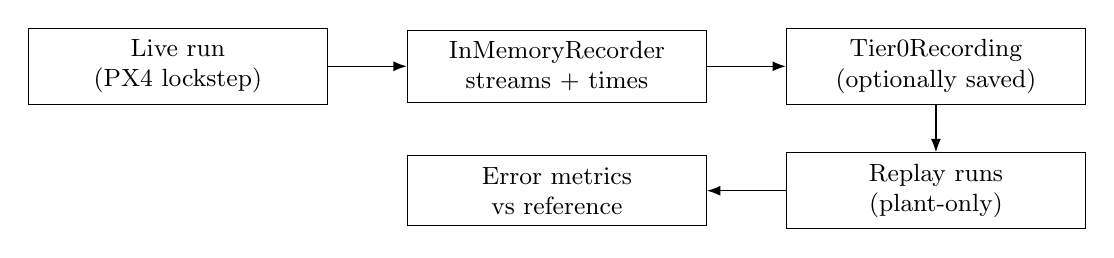
\begin{tikzpicture}[
      node distance=6mm and 10mm,
      font=\small,
      box/.style={draw, align=center, minimum width=38mm, inner ysep=4pt, inner xsep=6pt},
      arr/.style={-Latex, line width=0.4pt}
    ]
    \node[box] (live) {Live run\\(PX4 lockstep)};
    \node[box, right=of live] (rec) {\code{InMemoryRecorder}\\streams + times};
    \node[box, right=of rec] (tier0) {\code{Tier0Recording}\\(optionally saved)};
    \node[box, below=of tier0] (replay) {Replay runs\\(plant-only)};
    \node[box, left=of replay] (metrics) {Error metrics\\vs reference};
    \draw[arr] (live) -- (rec);
    \draw[arr] (rec) -- (tier0);
    \draw[arr] (tier0) -- (replay);
    \draw[arr] (replay) -- (metrics);
  \end{tikzpicture}
  \caption{Record/replay workflow: a single PX4 live run records boundary-aligned streams which are then reused to replay the plant under different integrators or plant variants.}
  \label{fig:record-replay-pipeline}
\end{figure}

\subsection{Trace representation}
\label{sec:trace-model}

Recorded streams are represented as typed traces indexed by an explicit integer-microsecond axis (\code{src/sim/Recording/Traces.jl}). The implementation provides three sampling semantics:
\begin{itemize}[leftmargin=*,itemsep=2pt]
  \item \textbf{\code{SampledTrace}}: defined only at exact axis times; sampling throws if the query time does not match an axis element.
  \item \textbf{\code{ZOHTrace}}: zero-order hold; sampling at time $t$ returns the most recent sample with time $\le t$.
  \item \textbf{\code{SampleHoldTrace}}: identical lookup to \code{ZOHTrace} but used to communicate ``sample-and-hold input'' intent (notably wind forcing).
\end{itemize}
All sampling is a deterministic binary search over the stored axis vector.

\subsection{Recorder and axis validation}

The default recorder is \code{Recording.InMemoryRecorder} (\code{src/sim/Recording/Recorder.jl}). It stores, for each named stream, a vector of timestamps and a vector of values.

\paragraph{Record-time checks.}
Each stream enforces nondecreasing timestamps (monotone time). It intentionally does \emph{not} require that every recorded timestamp belongs to a particular axis; that contract is validated when a trace is constructed.

\paragraph{Trace-build checks.}
When converting streams into traces, helpers such as \code{zoh\_trace(rec, name, axis)} validate that the recorded timestamps match the expected engine axis \emph{exactly} (\code{_require\_axis\_match!}). This is a fail-fast guard: ``almost aligned'' recordings do not silently produce incorrect sample-and-hold behavior.

\subsection{What is recorded in \texorpdfstring{\code{mode=:record}}{mode=:record}}
\label{sec:recorded-streams}

Record mode is implemented in the canonical engine loop (\code{src/sim/Runtime/Engine.jl}) via explicit \code{record!(recorder, name, t\_us, value)} calls at boundary stages.

\paragraph{Tier-0 streams.}
The helper \code{Recording.tier0\_traces} builds a minimal bundle sufficient for plant-only replay:
\begin{itemize}[leftmargin=*,itemsep=2pt]
  \item \code{:cmd} (\code{ActuatorCommand}) recorded on the autopilot axis and replayed with ZOH semantics.
  \item \code{:wind\_base\_ned} (\code{Vec3}) recorded on the wind axis and replayed as sample-and-hold.
  \item \code{:plant}, \code{:battery}, \code{:batteries} recorded on the log axis as exact samples.
\end{itemize}

\paragraph{Scenario streams.}
The engine can also record scenario outputs (arm/mission/RTL command, landed flag, faults, and optional wind disturbance). Two recording layouts exist (\code{src/sim/Recording/Recorder.jl}):
\begin{itemize}[leftmargin=*,itemsep=2pt]
  \item \textbf{Event-axis recording} (keys \code{*\_evt} on \code{timeline.evt}): enabled by \code{EngineConfig.record\_faults\_evt=true} (default in \code{Sim.simulate}). This captures scenario changes at the earliest possible hybrid boundary.
  \item \textbf{Scenario-axis recording} (keys without suffix on \code{timeline.scn}): used when event-axis recording is disabled.
\end{itemize}

\begin{table}[t]
  \centering
  \small
  \begin{tabular}{@{}llll@{}}
    \toprule
    Stream key & Value type & Axis & Trace semantics \\
    \midrule
    \code{:cmd} & \code{ActuatorCommand} & \code{ap} & \code{ZOHTrace} \\
    \code{:wind\_base\_ned} & \code{Vec3} & \code{wind} & \code{SampleHoldTrace} \\
    \code{:plant} & \code{PlantState} & \code{log} & \code{SampledTrace} \\
    \code{:battery} & \code{BatteryStatus} & \code{log} & \code{SampledTrace} \\
    \code{:batteries} & \code{Vector\{BatteryStatus\}} & \code{log} & \code{SampledTrace} \\
    \code{:ap\_cmd\_evt}, \code{:landed\_evt}, \code{:faults\_evt} & scenario outputs & \code{evt} & \code{ZOHTrace} \\
    (optional) \code{:wind\_dist\_evt} & \code{Vec3} & \code{evt} & \code{ZOHTrace} \\
    (optional) \code{:est} & \code{EstimatedState} & \code{ap} & \code{ZOHTrace} \\
    \bottomrule
  \end{tabular}
  \caption{Primary recorded streams and how they are replayed. ``Tier-0'' refers to the minimal set required to replay plant dynamics without stepping PX4.}
  \label{tab:recorded-streams}
\end{table}

\begin{figure}[t]
  \centering
  \includegraphics[width=\linewidth]{figs/record_vs_replay_overlay.png}
  \caption{Record/replay overlay for a single axis (position \(z\)) comparing the reference replay (RK45) to a replay with RK4.}
  \label{fig:record-vs-replay}
\end{figure}

\paragraph{Log snapshots are pre-step.}
When the log axis is due, the engine records the current plant state and battery telemetry \emph{before} integrating the next interval (see the \code{due\_log} block in \code{process\_events\_at!}). As a result, \code{:plant[k]} corresponds to the boundary state at \code{timeline.log.t\_us[k]}.

\subsection{Replay builds}

Replay runs are ordinary engine runs where live sources are replaced by trace-based sources:
\begin{itemize}[leftmargin=*,itemsep=2pt]
  \item \code{Sources.ReplayAutopilotSource} publishes recorded \code{bus.cmd} (ZOH on \code{timeline.ap}).
  \item \code{Sources.ReplayWindSource} publishes recorded base wind (sample-and-hold on \code{timeline.wind}).
  \item \code{Sources.ReplayScenarioSource} (optional) publishes recorded \code{bus.ap\_cmd}, \code{bus.landed}, \code{bus.faults}, and \code{bus.wind\_dist\_ned}.
\end{itemize}
To avoid double-forcing, the replay environment disables the live wind model (\code{Environment.NoWind}); all wind forcing comes from the recorded trace plus any replayed disturbance applied at event boundaries (\cref{sec:runtime-boundary}).

\subsection{Integrator sweep workflow}
\label{sec:integrator-sweep}

The workflow \code{Workflows.RecordReplay.compare\_integrators\_recording} runs a reference replay and then replays the same recording under a solver sweep:\vspace{-2pt}
\begin{enumerate}[leftmargin=*,itemsep=2pt]
  \item Build replay sources from the recording (Tier-0 traces, plus scenario traces if required).
  \item Run a \emph{reference} plant replay on the same \code{timeline} and \code{plant0}, recording \code{:plant} and \code{:battery} on the log axis.
  \item For each candidate solver, rerun the plant replay and compute error series vs the reference trajectory.
\end{enumerate}
The default reference integrator is an RK45 instance with tighter tolerances than the nominal Iris config (\code{_default\_reference\_integrator()} in \code{src/Workflows/RecordReplay.jl}). Error metrics are computed by \code{Verification.error\_series} (\code{src/sim/Verification.jl}) and reported as max norms over the log-axis samples.

\paragraph{Iris convenience wrapper.}
\code{Workflows.RecordReplay.compare\_integrators\_iris\_mission} combines:
\begin{itemize}[leftmargin=*,itemsep=2pt]
  \item an optional PX4 live record run via \code{Workflows.simulate\_iris\_mission(mode=:record)},
  \item reconstruction of the replay plant model from the TOML spec, and
  \item a plant-only replay sweep with optional CSV output.
\end{itemize}

\subsection{Determinism caveats}

The recording format is Julia \code{Serialization} (\code{Recording.write\_recording}/\code{read\_recording}). To reduce foot-guns, a schema version field (\code{BUS\_SCHEMA\_VERSION}) is checked at load time. Nevertheless, recordings should be treated as best-effort artifacts: they are intended for within-repository regression and integrator envelope validation, not as a stable long-term interchange format.

Finally, a \code{Tier0Recording} intentionally does not persist the full plant model or spec. Plant-only replay therefore assumes you rebuild the same \code{dynfun} (and consistent parameters) used to generate the recording.


\subsection{TOML configuration: run modes and recording I/O}
\label{sec:run-toml}

Record/replay behavior is selected in the \code{[run]} block (\code{RunSpec} in \code{src/sim/Aircraft/Spec.jl}):

\begin{lstlisting}[language=toml]
[run]
mode = "lockstep"        # "lockstep" or "replay"
recording_out = "run.jls"  # optional; if set, writes a recording
recording_in  = "run.jls"  # used only when mode="replay"
log_csv = "log.csv"         # optional; if set, writes a CSV log
\end{lstlisting}

\paragraph{Semantics.}
\begin{itemize}[leftmargin=*,itemsep=2pt]
  \item \code{mode}: selects whether PX4 is stepped live (\code{"lockstep"}) or whether the simulator consumes a previously recorded input/bus stream (\code{"replay"}).
  \item \code{recording\_out}: when non-null, the engine serializes the replayable boundary stream at the end of each run.
  \item \code{recording\_in}: path to a previously recorded stream; required for replay.
  \item \code{log\_csv}: optional human-readable CSV output independent of the replay stream.
\end{itemize}

\section{Validation and regression checks}
\label{sec:validation}

The simulator is intended to be reviewable and falsifiable: core claims are backed by executable tests in the repository. This section summarizes the current verification coverage and the contracts it enforces.

\subsection{Test harness}

The package test entrypoint is \code{test/runtests.jl}. A typical local invocation is:
\begin{lstlisting}
julia --project -e 'using Pkg; Pkg.test()'
\end{lstlisting}

The test suite is designed to run without a PX4 shared library. Lockstep runtime smoke tests (\code{test/integration/lockstep_runtime.jl}) are conditionally executed only when the lockstep library is available (see the \code{PX4Lockstep.has_lockstep()} gate).

\subsection{Analytic integrator verification}

The module \code{Sim.Verification} defines closed-form or invariant-rich reference problems, used in \code{test/verification/verification_cases.jl}:
\begin{itemize}[leftmargin=*,itemsep=2pt]
  \item \textbf{Simple harmonic oscillator (SHO).} With \code{dt=0.01} over \code{T=1.0}, RK4 is required to match the analytic position to \(<10^{-6}\). An additional regression checks that adaptive RK45 with \code{quantize_us=true} does not drift the requested timebase.
  \item \textbf{Pendulum.} For a small-angle case, RK4 must match the small-angle analytic solution to \(<10^{-5}\) and conserve energy to relative error \(<10^{-4}\) over one period.
  \item \textbf{Circular Kepler orbit.} RK4 must return to the analytic state after one orbit (at \(T_{end}=n\,dt\)) to \(<10^{-5}\) in position/velocity and conserve energy and angular momentum to \(<10^{-6}\) relative error.
  \item \textbf{Torque-free rigid body.} RK4 must conserve rotational energy to \(<10^{-6}\) relative error, keep quaternion norm within \(<10^{-10}\), and keep inertial angular momentum nearly constant.
\end{itemize}
These tests make the integrator implementations (\cref{sec:plant-state}) directly falsifiable.

\subsection{Representative verification results}
\label{sec:validation-results}

In addition to the unit-test style checks above, we periodically run standalone verification scripts under \code{Tools/px4\_lockstep\_julia/examples/verification/} to obtain concrete error magnitudes for common reference problems. \Cref{tab:verification-analytic-results} summarizes one such run.

\begin{table}[t]
  \centering
  \small
  \begin{tabular}{@{}llrr@{}}
    \toprule
    Case & Solver & Max error & Invariant drift \\
    \midrule
    SHO (\(\omega_0=2\pi\), \(T=1\,\mathrm{s}\), \(dt=0.01\)) & RK4  & $4.27\times 10^{-8}$  & $\Delta E/E=8.54\times 10^{-8}$ \\
    SHO (adaptive) & RK23 & $9.27\times 10^{-10}$ & $\Delta E/E=1.85\times 10^{-9}$ \\
    SHO (adaptive) & RK45 & $1.31\times 10^{-10}$ & $\Delta E/E=2.62\times 10^{-10}$ \\
    \midrule
    Pendulum (small angle, \(dt=0.01\)) & RK4  & $3.65\times 10^{-6}$ & $\Delta E/E=2.62\times 10^{-9}$ \\
    Pendulum (adaptive) & RK23 & $3.65\times 10^{-6}$ & $\Delta E/E=1.19\times 10^{-8}$ \\
    Pendulum (adaptive) & RK45 & $3.65\times 10^{-6}$ & $\Delta E/E=1.67\times 10^{-9}$ \\
    \midrule
    Kepler (circular, \(T=2\pi\), \(dt=0.01\)) & RK4  & $1.52\times 10^{-9}$ & $\Delta E/E=1.75\times 10^{-11}$ \\
    Kepler (circular, adaptive) & RK23 & $9.97\times 10^{-10}$ & $\Delta E/E=2.07\times 10^{-10}$ \\
    Kepler (circular, adaptive) & RK45 & $3.67\times 10^{-10}$ & $\Delta E/E=1.15\times 10^{-10}$ \\
    \midrule
    Rigid body (torque-free, \(dt=0.001\)) & RK4  & $|\Delta L|=5.81\times 10^{-12}$ & $\Delta E/E=4.94\times 10^{-14}$ \\
    Rigid body (torque-free, adaptive) & RK23 & $|\Delta L|=7.55\times 10^{-10}$ & $\Delta E/E=1.16\times 10^{-10}$ \\
    Rigid body (torque-free, adaptive) & RK45 & $|\Delta L|=5.11\times 10^{-10}$ & $\Delta E/E=4.76\times 10^{-11}$ \\
    \bottomrule
  \end{tabular}
  \caption{Representative analytic/invariant-rich verification results from standalone scripts. ``Max error'' is the final-state analytic deviation at \(T_{end}=n\,dt\) for SHO/pendulum/Kepler, and $|\Delta L|$ is the inertial angular-momentum change for the torque-free rigid-body case.}
  \label{tab:verification-analytic-results}
\end{table}

The same scripts include reference-compare problems that exercise full \code{PlantState} integration (rotor speed and battery states) against a tighter RK45 reference, as well as an end-to-end Iris record/replay integrator sweep. One such sweep (\(t_{end}=60\,\mathrm{s}\), \(\Delta t_{ap}=0.004\,\mathrm{s}\), \(\Delta t_{wind}=0.001\,\mathrm{s}\), \(\Delta t_{log}=0.01\,\mathrm{s}\)) reported the max errors in \cref{tab:verification-iris-sweep} relative to a reference replay.

\begin{table}[t]
  \centering
  \small
  \begin{tabular}{@{}lrrrrrr@{}}
    \toprule
    Solver & pos & vel & att & $\omega$ & rotor $\omega$ & $|\Delta I|$ \\
    \midrule
    RK4  & $7.52\times 10^{-5}$  & $4.14\times 10^{-6}$ & $7.30\times 10^{-8}$ & $2.24\times 10^{-7}$ & $1.15\times 10^{-4}$ & $2.92\times 10^{-6}$ \\
    RK23 & $6.37\times 10^{-4}$  & $2.96\times 10^{-5}$ & $2.62\times 10^{-7}$ & $2.49\times 10^{-6}$ & $1.61\times 10^{-3}$ & $6.98\times 10^{-5}$ \\
    RK45 & $0$ & $0$ & $4.21\times 10^{-8}$ & $0$ & $0$ & $0$ \\
    \bottomrule
  \end{tabular}
  \caption{Representative Iris record/replay integrator sweep: max error vs a reference replay trajectory. Columns correspond to the logged max norms used by \code{Workflows.RecordReplay.compare\_integrators\_recording} (position/velocity/attitude/body rates/rotor speed and battery-current error $|\Delta I|$).}
  \label{tab:verification-iris-sweep}
\end{table}

\begin{figure}[t]
  \centering
  \includegraphics[width=\linewidth]{figs/integrator_sweep_errors.png}
  \caption{Integrator sweep errors (log scale) for the same Iris record/replay run summarized in \cref{tab:verification-iris-sweep}.}
  \label{fig:integrator-sweep-errors}
\end{figure}

\subsection{Plant-level contract tests}

The file \code{test/verification/verification_contracts.jl} contains deterministic ``contract'' tests for the full multirotor plant and power system:
\begin{itemize}[leftmargin=*,itemsep=2pt]
  \item \textbf{Free-fall kinematics.} With motors off and no contact, the logged vertical position/velocity must match the closed-form constant-acceleration solution at \code{atol=1e-7} and maintain quaternion normalization.
  \item \textbf{Hover force-balance (RHS).} A single RHS evaluation is checked by solving for a rotor speed that yields total thrust \(\approx m g\) at sea-level density, then asserting vertical acceleration is \(\approx 0\) at identity attitude.
  \item \textbf{Power-bus solve fixed point.} A deterministic sweep over randomized rotor speeds/duties checks the bus-voltage solver returns a consistent fixed-point residual.
  \item \textbf{State sanity.} Logged states are asserted finite and within physical bounds (e.g. SOC \(\in[0,1]\), rotor speeds non-negative up to tolerance).
\end{itemize}

\subsection{Record/replay invariants}

The record/replay machinery is covered by \code{test/verification/record_replay_engine.jl}. These tests exercise:
\begin{itemize}[leftmargin=*,itemsep=2pt]
  \item axis-matching: building traces from a recording throws if recorded timestamps do not match the expected engine axis exactly,
  \item serialization schema enforcement through \code{BUS_SCHEMA_VERSION}, and
  \item replay determinism for Tier-0 streams (commands and wind) under multiple integrators.
\end{itemize}

\subsection{uORB injection tests}

The uORB injection scheduler and default state injector are covered by \code{test/uorb/uorb_injection.jl}, including multi-instance battery publishing behavior and the periodic ``due'' logic.

\subsection{Gaps and recommended extensions}

The current suite does not yet provide strong, closed-loop PX4 trajectory validation inside this repository (the lockstep runtime tests are intentionally minimal and are skipped when the PX4 shared library is unavailable). In practice, the most useful regression to add is a canonical PX4 mission recorded once and replayed under a solver sweep (\cref{sec:integrator-sweep}) with a saved CSV error summary.

\begin{figure}[t]
  \centering
  \includegraphics[width=\linewidth]{figs/mission_validation_xy_alt.png}
  \caption{Representative closed-loop Iris mission trace from a lockstep run (XY trajectory and altitude vs time). This is provided as a qualitative sanity check rather than a strict regression.}
  \label{fig:mission-validation}
\end{figure}

\section{Extension points}
\label{sec:extension-points}

Although the default Iris workflow is ``batteries + multirotor plant + wind + PX4 lockstep'', the codebase is structured around a small number of explicit interfaces. Extending the simulator is primarily a matter of implementing additional methods for these interfaces rather than modifying the engine.

\subsection{Discrete-time sources}

All discrete-time components that publish into the canonical signal bus (scenario, wind, estimator, autopilot) implement the runtime protocol:
\begin{quote}\small
\code{Runtime.update!(src, bus, plant_state, t_us)}
\end{quote}
The default fallback is a loud error (\code{Runtime.Engine.jl}) to avoid silent mis-wiring.

Sources that introduce additional event boundaries (typically scenarios) may also extend:
\begin{quote}\small
\code{Runtime.event_times_us(src, t0_us, t_end_us)}
\end{quote}
These event times are merged into the hybrid timeline by \code{Runtime.build_timeline_for_run}.

\paragraph{Determinism guideline.}
Sources are the intended home for randomness. They should draw randomness exclusively from explicit RNG state (seeded from \code{AircraftSpec.aircraft.seed}) and should never consult wall-clock time.

\subsection{Plant models and outputs}

A plant model is a callable RHS functor used by the integrator:
\begin{quote}\small
\code{dx = model(t::Float64, x::PlantState, u::PlantInput)}
\end{quote}
The engine treats the RHS as pure (no side effects) and therefore assumes it is deterministic given \((t,x,u)\).

Plants may optionally implement additional hooks (\code{src/sim/PlantInterface.jl}):
\begin{itemize}[leftmargin=*,itemsep=2pt]
  \item \code{plant_outputs(model, t, x, u)}: compute algebraic telemetry (forces, thrust, power, contact info) for logging and bus publication at event boundaries.
  \item \code{plant_project(model, x)}: enforce invariants after integration (e.g. quaternion renormalization, rotor speed clamping, contact post-stabilization).
  \item \code{plant_on_autopilot_tick(model, x, cmd)}: boundary-time discontinuities that must occur exactly at autopilot ticks (e.g. snapping \code{DirectActuators} outputs to the newly published command).
  \item \code{plant_integrate_interval(model, integrator, t0_us, x0, u, dt_us)}: optional hybrid interval stepping that can localize internal events (e.g. contact time-of-impact) and apply an impact map inside the interval.
\end{itemize}

\subsection{Contact models}

Ground/contact interaction is factored as a contact model (\code{src/sim/Contacts.jl}) attached to \code{PlantSpec.contact}. New models subtype \code{Contacts.AbstractContactModel} and (at minimum) implement a contact-to-world-force mapping at the vehicle COM:
\begin{quote}\small
\code{F_contact_ned = Contacts.contact_force_ned(model, rb_state, t)}
\end{quote}
where \code{rb_state} is the current rigid-body state (NED position/velocity + attitude + body rates). Models may additionally implement
\begin{quote}\small
\code{ci = Contacts.contact_info(model, rb_state, t)}
\end{quote}
to expose a \code{ContactInfo} snapshot (gap/penetration, contact mode, normal/friction force estimates) for logging and diagnostics.

For the unilateral constraint model \code{FlatGroundConstraintContact}, the normal reaction depends on the \emph{unconstrained} acceleration; it is therefore evaluated with the overload
\begin{quote}\small
\code{F_contact_ned = Contacts.contact_force_ned(model, rb_state, t, mass, a_free_ned)}
\end{quote}
used by the plant outputs layer.

Hybrid touchdown/bounce handling is implemented at the plant level via \code{plant_integrate_interval(...)} (e.g. time-of-impact localization + impact map for flat-ground contact). The default Iris spec uses \code{flat_ground_constraint} contact.

\subsection{PX4 uORB injection sources}


PX4 lockstep integration is mediated through a uORB injector. See \code{src/sim/Autopilots/UORBInjection.jl}. The injector owns a list of \code{AbstractUORBInjectionSource} objects. Each source can publish at a declared integer-microsecond cadence via:
\begin{quote}\small
\code{inject_due!(src, handle, ctx, t0_us)}
\end{quote}
A convenience implementation \code{PeriodicUORBInjection} is provided: users supply a topic-specific message builder \code{builder(ctx)} and configure its \code{period_us} and \code{phase_us}. The default Iris workflow uses the built-in state injector \code{build_state_injection_injector}.

\section{Related work and positioning}
\label{sec:related-work}

This paper is primarily an implementation description, but it is still useful to position the design against common autopilot-in-the-loop practice. We keep this section intentionally high-level in the current draft; a camera-ready version should add formal citations.

\subsection{SITL and lockstep autopilot integration}

PX4 SITL deployments commonly pair the autopilot with an external simulator that advances ``time'' in some form and exchanges state/actuator topics. In many stacks the simulator attempts to run in (scaled) real time, and the autopilot is advanced in a loop that is ultimately coupled to wall-clock scheduling. \code{PX4Lockstep.jl} instead treats PX4 as a discrete-time component stepped on an injected clock: the simulation engine never advances PX4 by wall time, and the boundary ordering is part of the explicit semantics (\cref{sec:runtime-boundary}).

\subsection{Physics engines vs. reviewable determinism}

High-fidelity physics engines and robotics simulators provide rich contact and aerodynamics models, but they frequently trade away strict repeatability due to internal multi-threading, nondeterministic collision ordering, and floating-point reductions. The design goal here is deliberately different: to make the execution model and the determinism boundary reviewable, and to keep the ``truth'' models small enough that equations, defaults, and corner cases can be documented code-faithfully.

\subsection{Deterministic hybrid simulation and record/replay}

The union-event-axis execution model is closely related in spirit to deterministic discrete-event simulation: subsystems publish changes only at explicitly scheduled boundaries and the continuous state advances deterministically between them. Record/replay then becomes a natural scientific tool: a closed-loop run can be reduced to boundary-aligned input traces and replayed as an open-loop plant experiment (\cref{sec:record-replay}). This mirrors ``record and replay'' ideas used in systems debugging, but the emphasis here is on plant-side falsifiability: any divergence under replay is attributable to plant/integrator/model changes, not controller behavior.

\paragraph{Citations.}
Formal citations are intentionally deferred in this draft. A camera-ready revision should cite: (i) canonical PX4 SITL simulators and lockstep interfaces, (ii) deterministic hybrid simulation frameworks/discrete-event semantics, and (iii) record/replay systems for reproducibility and debugging. These citations are not load-bearing for understanding the implementation described here.

\section{Nonstandard modeling choices and rationale}
\label{sec:design-choices}

This simulator is optimized for deterministic regression and rapid iteration. A few modeling choices intentionally diverge from common aerospace references; they are not ``wrong,'' but they should be read as pragmatic tradeoffs rather than canonical physics. The list below records these choices and the intended future direction.

\subsection{Local NED-to-LLA approximation}
The NED-to-LLA conversion used for PX4 topic injection is a flat-Earth approximation with a fixed \(\cos(\varphi_0)\) longitude scale and linear altitude (\cref{sec:home-origin}). This is adequate for local missions (order \(\sim\)\SI{10}{km} from home) and deterministic regression, but it is not suitable for large-area navigation or high-latitude operations. A future extension could substitute a proper geodesic conversion or an Earth-centered frame.

\subsection{Turbulence model: OU vs. Dryden/Von K\'arm\'an}
The wind model uses an Ornstein--Uhlenbeck (OU/AR(1)) process (\cref{sec:wind}) rather than a Dryden or Von K\'arm\'an spectral model. OU is chosen because it is simple, strictly Markov, and deterministic under fixed random seeds, making it attractive for regression. It does not attempt to match turbulence power spectra used in certification-oriented literature. If spectral fidelity becomes a goal, Dryden/Von K\'arm\'an parameterizations should be added as alternative wind sources.

\subsection{State injection instead of raw sensor simulation}
The default lockstep bridge injects filtered state estimates into PX4 rather than simulating raw sensors and running an onboard estimator (\cref{sec:px4-bridge}, \cref{sec:limitations}). This provides stable, deterministic closed-loop regression but does not exercise estimator failure modes or sensor bandwidth limitations.

\subsection{Simplified contact and aerodynamics}
Ground contact is modeled as a single COM contact with a hybrid impact map and an impulse-based grounded solve (\cref{sec:contacts}). This is in the family of time-stepping / complementarity-inspired rigid-contact methods (e.g., Stewart--Trinkle 1996; Anitescu--Potra 1997), but implemented in a minimal single-contact form for determinism. Aerodynamics are linear drag only (\cref{sec:rigid-body}). These choices prioritize stability and determinism; they are not intended to represent landing gear dynamics or aerodynamic performance.

\subsection{Ad-hoc prop inflow attenuation}
The propeller inflow correction uses a simple \(\mu^2\) attenuation \(f(\mu)=1/(1+k\mu^2)\) (\cref{sec:propulsion-model}). This is a pragmatic shaping term (not a blade-element or momentum-theory model) and ignores the sign of axial velocity. It therefore cannot represent windmilling, vortex-ring, or braking regimes.

\section{Known limitations and improvement targets}
\label{sec:limitations}

This section lists limitations that are \emph{explicit in the code} and therefore matter when interpreting results.

\subsection{State injection rather than raw sensor simulation}
The default PX4 integration uses ``state injection'' uORB topics published at every PX4 step (\code{src/sim/Autopilots/UORBInjection.jl}), not raw IMU/mag/baro/GPS measurements. The estimator layer therefore models ``EKF output error'' rather than sensor physics.

\subsection{Aerodynamics are intentionally minimal}
The rigid-body drag model is linear and isotropic (\code{Vehicles.GenericMultirotor}); it does not include lift, induced drag, rotor/airframe aerodynamic coupling, blade flapping, or ground effect. Propulsor inflow is captured only through a simple $\mu^2$ attenuation factor on thrust/torque (\cref{sec:propulsion-model}).

\subsection{Contacts are COM forces only}
The shipped ground models (\code{FlatGroundContact} and \code{FlatGroundConstraintContact}) apply contact at the vehicle center of mass (COM) and therefore produce no moments. While \code{FlatGroundConstraintContact} includes deterministic hybrid impact handling (time-of-impact localization + restitution/impact friction) and a fixed-step grounded impulse solve for stable resting contact, it is still not a landing-gear or multi-point contact model. Energy and angular-momentum conservation are not enforced (normal velocity is reset, tangential velocity is clamped by Coulomb bounds, and there is no angular impulse). Terrain heightfields and contact-induced torques remain out of scope for the current contact layer.

\subsection{No regeneration / no charging}
The BLDC current model clamps negative current to zero, and the battery model integrates only discharge current ($I\gets\max(0,I)$). There is no regenerative braking, motor back-driving into the bus, or battery charging model.

\subsection{Power-network topology is intentionally simple}
\code{PowerNetwork} supports only ``battery belongs to a bus'' wiring with per-bus constant-power avionics loads. Cross-feed, diode OR-ing, and richer circuit effects are intentionally out of scope. Additionally, avionics constant-power load is approximated as a constant current during the bus-voltage solve (\cref{sec:bus-solve}).

\subsection{Static scenario event discovery}
The hybrid timeline can include scenario \code{AtTime} events discovered from a static scheduler. Dynamically inserting new events at runtime is not supported by the current timeline builder.

\subsection{Geodesy and gravity approximations}
The NED$\leftrightarrow$LLA conversion used for PX4 topic injection is a local flat-Earth approximation (fixed \(\cos(\varphi_0)\) longitude scale and linear altitude). It is intended for missions within \(\sim\)\SI{10}{km} of the home origin. \code{SphericalGravity} treats local down as radial with $r\approx r_0 - z$. These are appropriate for short-range missions around the home origin but not for large-area navigation studies.

\subsection{Floating-point and environment-dependent determinism}
While the runtime semantics are deterministic at the event-scheduling layer (integer timebase, fixed boundary ordering), bitwise-identical results are not guaranteed across different floating-point environments. Multi-threaded dependencies, different \code{libm} implementations, CPU instruction sets (e.g. fused multiply-add behavior), or dependency version drift can all change rounding and therefore plant trajectories. The project currently targets repeatability \emph{within a controlled environment}; the threat model and recommended controls are stated explicitly in \cref{sec:determinism-threat-model}.


\appendix
\section{Default Iris spec (TOML assets)}
\label{app:iris}

The repository ships a TOML-first default Iris configuration:
\begin{itemize}[leftmargin=*,itemsep=2pt]
  \item \code{src/Workflows/assets/aircraft/iris\_default.toml}: mission timing, plant/environment, airframe, actuation, and power.
  \item \code{src/Workflows/assets/aircraft/iris\_uorb.toml}: the uORB interface contract (topics to publish/subscribe).
\end{itemize}
The default spec uses \code{extends=["iris\_uorb.toml"]}; the loader deep-merges these files (\cref{sec:configuration}).

This appendix summarizes the key resolved parameters of the default Iris spec.

\subsection{Home origin and PX4 configuration}

\begin{table}[ht]
  \centering
  \small
  \begin{tabular}{@{}p{0.44\textwidth}p{0.50\textwidth}@{}}
    \toprule
    \textbf{Field} & \textbf{Value} \\
    \midrule
    \code{home.lat\_deg} & 47.397742 \\
    \code{home.lon\_deg} & 8.545594 \\
    \code{home.alt\_msl\_m} & \SI{488.0}{m} \\
    \midrule
    \code{px4.mission\_path} & \code{../missions/simple\_mission.waypoints}\\(relative to \code{iris\_default.toml}) \\
    \code{px4.edge\_trigger} & \code{false} \\
    \code{px4.derive\_ca\_params} & \code{true} \\
    \code{px4.libpath} & \emph{unset in the shipped asset (required for live/record)} \\
    \bottomrule
  \end{tabular}
  \caption{Home origin and PX4 configuration defaults. Relative paths resolve against the spec file directory.}
\end{table}

\begin{table}[ht]
  \centering
  \small
  \begin{tabular}{@{}p{0.44\textwidth}p{0.50\textwidth}@{}}
    \toprule
    \textbf{PX4 lockstep field} & \textbf{Value} \\
    \midrule
    \code{dataman\_use\_ram} & 1 \\
    \code{enable\_commander} & 0 \\
    \code{commander\_rate\_hz} & 100 \\
    \code{navigator\_rate\_hz} & 20 \\
    \code{mc\_pos\_control\_rate\_hz} & 100 \\
    \code{mc\_att\_control\_rate\_hz} & 250 \\
    \code{mc\_rate\_control\_rate\_hz} & 250 \\
    \code{enable\_control\_allocator} & 1 \\
    \code{control\_allocator\_rate\_hz} & 250 \\
    \bottomrule
  \end{tabular}
  \caption{Lockstep module rates from \code{[px4.lockstep]}.}
\end{table}

\subsection{Timeline, plant, and environment}

\begin{table}[ht]
  \centering
  \small
  \begin{tabular}{@{}p{0.44\textwidth}p{0.50\textwidth}@{}}
    \toprule
    \textbf{Field} & \textbf{Value} \\
    \midrule
    \code{timeline.t\_end\_s} & \SI{20.0}{s} \\
    \code{timeline.dt\_autopilot\_s} & \SI{0.004}{s} \\
    \code{timeline.dt\_wind\_s} & \SI{0.001}{s} \\
    \code{timeline.dt\_log\_s} & \SI{0.01}{s} \\
    \midrule
    \code{plant.integrator} & \code{RK45} \\
    \code{plant.contact} & \code{flat\_ground\_constraint} \\
    \midrule
    \code{environment.atmosphere} & \code{isa1976} \\
    \code{environment.gravity} & \code{uniform}, $g=\SI{9.80665}{m/s^2}$ \\
    \code{environment.wind} & \code{ou} \\
    \code{environment.wind\_mean\_ned} & $(0,0,0)$\,m/s \\
    \code{environment.wind\_sigma\_ned} & $(1.5,1.5,0.5)$\,m/s \\
    \code{environment.wind\_tau\_s} & \SI{3.0}{s} \\
    \bottomrule
  \end{tabular}
  \caption{Default timeline, plant selection, and environment parameters.}
\end{table}

\subsection{Scenario and estimator}

\begin{table}[ht]
  \centering
  \small
  \begin{tabular}{@{}p{0.44\textwidth}p{0.50\textwidth}@{}}
    \toprule
    \textbf{Field} & \textbf{Value} \\
    \midrule
    \code{scenario.arm\_time\_s} & \SI{1.0}{s} \\
    \code{scenario.mission\_time\_s} & \SI{2.0}{s} \\
    \midrule
    \code{estimator.kind} & \code{noisy\_delayed} \\
    \code{estimator.pos\_sigma\_m} & $(0.02,0.02,0.02)$\,m \\
    \code{estimator.vel\_sigma\_mps} & $(0.05,0.05,0.05)$\,m/s \\
    \code{estimator.yaw\_sigma\_rad} & 0.01 \\
    \code{estimator.rate\_sigma\_rad\_s} & $(0.005,0.005,0.005)$\,rad/s \\
    \code{estimator.bias\_tau\_s} & \SI{50.0}{s} \\
    \code{estimator.rate\_bias\_sigma\_rad\_s} & $(0.001,0.001,0.001)$\,rad/s \\
    \code{estimator.delay\_s} & \SI{0.008}{s} \\
    \code{estimator.dt\_est\_s} & \SI{0.004}{s} \\
    \bottomrule
  \end{tabular}
  \caption{Default scenario and estimator parameters.}
\end{table}

\subsection{Rigid body, geometry, and propulsion}

\begin{table}[ht]
  \centering
  \small
  \begin{tabular}{@{}p{0.44\textwidth}p{0.50\textwidth}@{}}
    \toprule
    \textbf{Field} & \textbf{Value} \\
    \midrule
    \code{airframe.mass\_kg} & \SI{1.5}{kg} \\
    \code{airframe.inertia\_diag\_kgm2} & $(0.029125,0.029125,0.055225)$\,kg\,m$^2$ \\
    \code{airframe.linear\_drag} & \SI{0.05}{N/(m/s)} \\
    \code{airframe.angular\_damping} & $(0.02,0.02,0.01)$ \\
    \midrule
    Rotor positions $\vect{r}_{b,i}$ (m) &
      $\{(0.1515,0.2450,0),\;(-0.1515,-0.1875,0),\newline
      (0.1515,-0.2450,0),\;(-0.1515,0.1875,0)\}$ \\
    Rotor axes $\vect{a}_{b,i}$ & $(0,0,1)$ for all four \\
    \midrule
    \code{propulsion.km\_m} & 0.05 \\
    \code{propulsion.V\_nom} & \SI{12.0}{V} \\
    \code{propulsion.rho\_nom} & \SI{1.225}{kg/m^3} \\
    \code{propulsion.rotor\_radius\_m} & \SI{0.127}{m} \\
    \code{propulsion.inflow\_kT}, \code{inflow\_kQ} & 8.0, 8.0 \\
    \code{propulsion.thrust\_calibration\_mult} & 2.0 \\
    \code{propulsion.rotor\_dir} & $(+1,+1,-1,-1)$ \\
    \midrule
    \code{esc.eta} & 0.98 \\
    \code{esc.deadzone} & 0.02 \\
    \midrule
    \code{motor.kv_rpm_per_volt} & 920 \\
    \code{motor.r_ohm} & \SI{0.25}{\ohm} \\
    \code{motor.j_kgm2} & $1.2\times 10^{-5}$\,kg\,m$^2$ \\
    \code{motor.i0_a} & \SI{0.6}{A} \\
    \code{motor.viscous_friction_nm_per_rad_s} & $2.0\times 10^{-6}$ \\
    \code{motor.max_current_a} & \SI{60}{A} \\
    \bottomrule
  \end{tabular}
  \caption{Default rigid-body, geometry, and propulsion parameters.}
\end{table}

\subsection{Actuation mapping and power network}

\begin{table}[ht]
  \centering
  \small
  \begin{tabular}{@{}p{0.44\textwidth}p{0.50\textwidth}@{}}
    \toprule
    \textbf{Field} & \textbf{Value} \\
    \midrule
    Motor channel map & $\{\texttt{motor1}\mapsto 1,\;\texttt{motor2}\mapsto 2,\;\texttt{motor3}\mapsto 3,\;\texttt{motor4}\mapsto 4\}$ \\
    \code{motor\_actuators.kind} & \code{direct} \\
    \code{servo\_actuators.kind} & \code{direct} \\
    \midrule
    \code{power.share\_mode} & \code{inv\_r0} \\
    \code{battery.model} & \code{thevenin} \\
    \code{battery.capacity\_ah} & \SI{5.0}{Ah} \\
    \code{battery.soc0} & 1.0 \\
    \code{battery.ocv} & linear: $10.8\to 12.6$\,V over SOC $0\to 1$ \\
    \code{battery.r0} & \SI{0.020}{\ohm} \\
    \code{battery.r1},\code{battery.c1} & $\SI{0.010}{\ohm}$, \SI{2000}{F} \\
    \code{battery.min\_voltage\_v} & \SI{9.9}{V} \\
    \code{battery.low/crit/emerg} & 0.15 / 0.10 / 0.05 \\
    \midrule
    Bus wiring & $\{\texttt{main}:\;\texttt{bat1}\to\texttt{motor1..4}\}$, avionics load $0$\,W \\
    \bottomrule
  \end{tabular}
  \caption{Default actuation mapping and power-network parameters (single bus, single battery).}
\end{table}

\paragraph{uORB contract.}
The default Iris uORB publish/subscribe set is defined in \code{iris\_uorb.toml}. The resulting state-injection topics and their units/frames are summarized in \cref{app:uorb-injection}.

\section{PX4 uORB injection contract}
\label{app:uorb-injection}

This appendix documents the concrete uORB messages injected by the simulator into PX4 in lockstep mode. The implementation lives in:
\begin{itemize}[leftmargin=*,itemsep=2pt]
  \item \code{src/sim/Autopilots/UORBBridge.jl} (message packing and uORB bridge), and
  \item \code{src/sim/Autopilots/UORBInjection.jl} (publish scheduling and state-to-message mapping).
\end{itemize}

\subsection{Injection call site}

PX4 is stepped once per autopilot tick through \code{Autopilots.autopilot\_step}. For each tick, the simulator:
\begin{enumerate}[leftmargin=*,itemsep=2pt]
  \item builds a \code{PX4StepContext} snapshot containing time, rigid-body state, estimated yaw, geodetic position, autopilot command, arming/nav state, and battery telemetry,
  \item calls \code{inject\_due!} to publish any uORB topics that are scheduled for the current time, and
  \item calls \code{step\_uorb!} to advance PX4's internal uORB graph by one lockstep step.
\end{enumerate}

\subsection{Default Iris interface}

The default Iris assets define the uORB interface contract in \code{iris\_uorb.toml}. The \emph{publisher} list describes what the simulator injects into PX4; the \emph{subscriber} list describes what the simulator reads back from PX4 after stepping.

\paragraph{Injected uORB topics (default Iris).}
The default state injector publishes each configured topic \emph{every PX4 step} (period $=0$). \cref{tab:uorb-pubs} lists the injected topics and their primary semantics.

\begin{table}[t]
  \centering
  \small
  \begin{tabularx}{\linewidth}{@{}l l >{\raggedright\arraybackslash}X@{}}
    \toprule
    Publisher key & uORB msg type & Notes (units / frames) \\
    \midrule
    \code{battery\_status} & \code{BatteryStatusMsg} & Multi-instance support; uses \code{ctx.batteries}. \\
    \code{vehicle\_attitude} & \code{VehicleAttitudeMsg} & Quaternion \(q_{bn}\) (Body$\to$NED), \(\omega_{body}\) in rad/s. \\
    \code{vehicle\_local\_position} & \code{VehicleLocalPositionMsg} & \(p_{ned}\) (m), \(v_{ned}\) (m/s), yaw (rad). \\
    \code{vehicle\_global\_position} & \code{VehicleGlobalPositionMsg} & Lat/Lon (deg), alt\_msl (m). \\
    \code{vehicle\_angular\_velocity} & \code{VehicleAngularVelocityMsg} & Body rates (rad/s). \\
    \code{vehicle\_land\_detected} & \code{VehicleLandDetectedMsg} & Uses \code{ctx.landed}. \\
    \code{vehicle\_status} & \code{VehicleStatusMsg} & Sets \code{nav\_state}, \code{arming\_state}. \\
    \code{vehicle\_control\_mode} & \code{VehicleControlModeMsg} & Enables attitude/rate/allocator booleans. \\
    \code{actuator\_armed} & \code{ActuatorArmedMsg} & Armed/prearmed based on \code{ctx.cmd.armed}. \\
    \code{home\_position} & \code{HomePositionMsg} & Publishes home LLA; gated on finite home values. \\
    \code{geofence\_status} & \code{GeofenceStatusMsg} & Sets \code{geofence\_violated=false}. \\
    \bottomrule
  \end{tabularx}
  \caption{Default Iris uORB publishers injected by the simulator (\code{iris\_uorb.toml}). Unless overridden by custom injection sources, all default topics publish every PX4 step.}
  \label{tab:uorb-pubs}
\end{table}

\paragraph{Subscribed uORB topics (default Iris).}
After each PX4 step, the bridge reads a fixed set of uORB subscriptions to construct the autopilot output bundle \code{UORBOutputs}. The default Iris list is:
\begin{quote}\small
\code{torque\_sp}, \code{thrust\_sp}, \code{actuator\_motors}, \code{actuator\_servos}, \code{attitude\_sp},\ \\
\code{rates\_sp}, \code{mission\_result}, \code{vehicle\_status}, \code{battery\_status}, \code{trajectory\_setpoint}.
\end{quote}

\paragraph{Actuator output normalization.}
The simulator interprets \code{actuator\_motors} as normalized ESC duty commands in \([0,1]\) and \code{actuator\_servos} as normalized control-surface deflections in \([-1,1]\). These are the lockstep ABI conventions used by \code{ActuatorCommand}; they are not PWM values. If a different uORB topic or scaling is desired (e.g.\ reversible motors), the mapping should be adjusted in the bridge and documented in the interface config.

\subsection{State-to-message mapping details}

This section highlights the non-obvious mapping choices that matter for correctness.

\paragraph{Attitude quaternion convention.}
\code{VehicleAttitudeMsg.q} is populated with \(q_{bn}\) (body$\to$NED), ordered as \((w,x,y,z)\) and normalized at parse-time in the TOML loader. See \cref{sec:frames} for the simulator frame conventions.

\paragraph{Local position reference.}
\code{VehicleLocalPositionMsg.ref\_lat/ref\_lon/ref\_alt} are chosen based on whether commander-in-loop is enabled. When \code{enable\_commander==0} (the Iris default), the reference is forced to the configured home location so PX4 receives a consistent local-frame origin.

\paragraph{Battery injection and instances.}
Battery status injection supports multiple uORB instances. If the interface config contains multiple \code{battery\_status} publishers with instances \(0,1,\dots\), the injector publishes one message per instance. Instance \(i\) maps to \code{ctx.batteries[i+1]}; missing batteries are rejected.

\subsection{Publish scheduling and cadence constraints}
\label{sec:uorb-scheduling}

Each injected topic is driven by an \code{AbstractUORBInjectionSource} with parameters:
\begin{itemize}[leftmargin=*,itemsep=2pt]
  \item \code{period\_us}: publish period in microseconds (\code{0} means ``every PX4 step''),
  \item \code{phase\_us}: phase offset relative to the injector's \code{t0\_us} (captured on first use).
\end{itemize}
For non-zero periods, a publish is \emph{due} at time \(t\) when \((t - t_0 - \phi) \bmod P = 0\) (see \code{_is\_due} in \code{UORBInjection.jl}).

\paragraph{Cadence validation.}
When running a live PX4 autopilot, \code{Sim.simulate} checks that periodic injection sources are compatible with the autopilot cadence:\vspace{-2pt}
\begin{itemize}[leftmargin=*,itemsep=2pt]
  \item the autopilot step \(\Delta t_{ap}\) must not be slower than the minimum declared injection period, and
  \item each declared injection period must be an integer multiple of \(\Delta t_{ap}\).
\end{itemize}
If an injection period is not a multiple of the autopilot cadence and strict checking is disabled, the simulator warns that scheduled publishes will be skipped (effective period becomes the least common multiple of \(P\) and \(\Delta t_{ap}\)).

\paragraph{Default Iris behavior.}
The built-in state injector sets all default topic periods to \code{0}, so the injection schedule does not constrain \(\Delta t_{ap}\) for the default Iris workflow.

\section{Run context for reported figures}
\label{app:run-context}

This appendix records the configuration used for the replay-only runtime figure (\cref{fig:replay-rtf}). The goal is to make the reported numbers reproducible without overloading the figure caption.

\subsection{Replay-only realtime factor (700 s mission)}

\begin{table}[ht]
  \centering
  \small
\begin{tabular}{@{}p{0.44\textwidth} >{\raggedright\arraybackslash}p{0.50\textwidth}@{}}
    \toprule
    \textbf{Field} & \textbf{Value} \\
    \midrule
    Spec path & \code{examples/specs/iris\_example\_3s2p\_10ah\_surface\_rc\_thermal\_lockstep.toml} \\
    Run mode & Replay-only sweep (no PX4 calls during replay) \\
    Recording source & \code{examples/replay/out_long/iris_long_tier0.jls} \\
    \midrule
    \(t_{end}\) & 700\,s \\
    \(\Delta t_{ap}\) & 0.004\,s \\
    \(\Delta t_{wind}\) & 0.001\,s \\
    \(\Delta t_{log}\) & 0.01\,s \\
    \midrule
    Integrators swept & RK4, RK23, RK45 (nominal tolerances) \\
    Reference integrator & RK45 (tight tolerances; \code{default reference integrator}) \\
    Contact model & \code{flat\_ground\_constraint} (hybrid) \\
    Battery model & Thevenin + surface R0(s,T), thermal enabled \\
    \bottomrule
  \end{tabular}
  \caption{Configuration context for the replay‑only realtime factor plot.}
  \label{tab:rtf-run-context}
\end{table}

The RTF values in \cref{fig:replay-rtf} are computed from the recorded mission duration (\(t_{end}\)) and the measured wall time of each replay. Because the replay sweep does not call into PX4, these timings reflect only the Julia‑side plant and engine cost.


\end{document}
